\documentclass[12pt,a4paper]{monografia}
\usepackage{amsfonts}
\usepackage{amsmath}
\usepackage{qtree}
\usepackage{siunitx}
\usepackage{acronym}
%\usepackage{amssymb}

%TODOS OS PACKAGE DEVEM SER COLOCADOS AKI
\usepackage[brazil,brazilian,portuges]{babel}
\usepackage[T1]{fontenc}
%\usepackage[brazilian]{babel}
\usepackage{mathptmx}

\usepackage{amsmath,listings,indentfirst,url,hyperref}
%\usepackage{amsmath,listings,indentfirst}
\usepackage{paralist}
\usepackage[all]{hypcap}
\usepackage[alf]{abntex2cite}
\usepackage[portuguese]{nomencl}
\usepackage{longtable}
\usepackage{fancyvrb}
\usepackage{color}
\usepackage{rotating}
\usepackage{multirow}
\usepackage{latexsym}
\usepackage[table]{xcolor}
\usepackage[utf8]{inputenc}
\usepackage[section]{placeins}
\usepackage{graphicx}
\usepackage{caption}
%%resize table op1
\usepackage{adjustbox}
%\usepackage{slashbox,booktabs,amsmath}
\usepackage{diagbox}
\usepackage{enumitem}
\usepackage{booktabs}
\usepackage{quoting}
\usepackage{setspace}
\usepackage[table]{xcolor}

\usepackage{subcaption} 
%só colocar 
%\adjustbox{max height=\dimexpr\textheight-5.5cm\relax,
%           max width=\textwidth}{
%antes do tabular 
%lembrar de fechar o { no \end{tabular} }


% pacotes de fontes! doi ter que usar times para evitar problemas :(
%\usepackage{fontspec}
%\usepackage{xunicode} 
%\defaultfontfeatures{Mapping=tex-text} 
%\setromanfont{Garamond}
%\setsansfont{Gill Sans}
%\setmonofont{Courier New}

% Listings
\lstset{
    inputencoding=utf8,
    basicstyle=\scriptsize,
    frame=single,
	tabsize=4,
	captionpos=b,
	breaklines=true,
	numbers=left,
}

% Não sei porque mas o LaTeX insiste em avançar a margem nas citações.
% Felizmente há o comando \sloppy, que diz para aumentar o espaçamento
% entre as palavras, visando /sempre/ respeitar as margens. Fica feio
% em alguns parágrafos, mas é a vida...
\sloppy

% da um trato nos floats
\renewcommand{\topfraction}{.85}
\renewcommand{\bottomfraction}{.7}
\renewcommand{\textfraction}{.15}
\renewcommand{\floatpagefraction}{.66}
\renewcommand{\dbltopfraction}{.66}
\renewcommand{\dblfloatpagefraction}{.66}
\setcounter{topnumber}{9}
\setcounter{bottomnumber}{9}
\setcounter{totalnumber}{20}
\setcounter{dbltopnumber}{9}

%\addto\captionsportuges{
%  \renewcommand{\tablename}
%    {Quadro}}

%\addto\captionsportuges{
%  \renewcommand{\listtablename}
%    {Lista de Quadros}}

\renewcommand{\lstlistingname}{C\'odigo}
\def\listofsymbols{\def\addsymbol #1 #2{#1  & \hspace{0.5in} #2 \\ } 

\begin{tabular}{l l}

% A
% B
% C
% D
% E
% F
% G
% H

%I
    
    \addsymbol IaaS {\textit{Infrastructure as a Service}}
% J
% K
% L
% M
% N
% O
% P
% Q
% R
% S
    \addsymbol SC {Contratos Inteligentes(\textit{Smart Contracts})}
% T
% U
% V
% W
% X
% Y
% Z

\end{tabular}

 \clearpage}

% Verbatim não precisa de espaçamento duplo e nem de fontes tão grandes
\RecustomVerbatimEnvironment
	{Verbatim}%
	{Verbatim}%
	{baselinestretch=1,	fontsize=\relsize{-1}}



%%%%%%%%%%%%%%count enumarete start in zero
\usepackage{enumitem}
\setlist[enumerate,1]{start=1} % only outer nesting level

%%%%%%%%cite inside enumerate
\makeatletter
\newcommand{\mylabel}[2]{#2\def\@currentlabel{#2}\label{#1}}
\makeatother


\hyphenation{re-co-nhe-ci-men-to}
\hyphenation{re-su-mi-da-men-te}
\hyphenation{in-vá-li-da}
\hyphenation{i-ma-gem}
\hyphenation{li-te-ra-tu-ra}
\hyphenation{ma-nu-al-men-te}
\hyphenation{re-pre-sen-ta}
\begin{document}
	\titulo{Alvorada: Protocolo baseado em Blockchain para Elaboração e Auditoria de Contratos entre Provedores de Microsserviços e Usuários}
\autor{Wilton Jaciel Loch}
\nome{Wilton Jaciel}
\ultimonome{Loch}


\bacharelado \curso{Ciência da Computação}
\ano{2019}
\data {\today}
\cidade{Joinville}

\instituicao{Universidade do Estado de Santa Catarina}
\sigla{UDESC}
\unidadeacademica{Centro de Ciências Tecnológicas}

\orientador{Prof. Guilherme Piêgas Koslovski}
\examinadorum{Prof. Charles Christian Miers}
\examinadordois{Prof. Maurício Aronne Pillon}

\ttorientador{Doutor}
\ttexaminadorum{Doutor}
\ttexaminadordois{Doutor}

\newpage
\pagestyle{empty}

\maketitle

%\begin{dedicatoria}
%\noindent
%\end{dedicatoria}
%\noindent
%\newpage
%\begin{epigrafe}
%\noindent
%\end{epigrafe}

%\agradecimento{Agradecimentos}
%caneta

\resumo{Resumo}
\noindent Os microsserviços são um modelo arquitetural cada vez mais utilizado no meio computacional. Suas vantagens, principalmente relacionadas à eficiência e escalabilidade quando comparado com o modelo monolítico, fazem com que seu uso seja visado por diversas empresas.
%
Contudo, a ampla adoção para implementação de serviços complexos e distribuídos requer a manipulação de requisições em larga escala.
%
Assim, torna-se necessária a seleção de provedores para alocar a execução dos microsserviços, bem como escalonar suas tarefas, de modo que atuem corretamente no âmbito das aplicações.
%
Um fator agravante no cenário em questão é a existência de múltiplos provedores, arquiteturalmente posicionados nas nuvens ou nas bordas da Internet, com diferentes preços, estratégias e qualidades nos seus serviços.
%
Tais provedores compõem um mercado heterogêneo e competitivo no qual adotam diferentes características do serviço.
%
Nesse ambiente, os contratos se estabelecem principalmente através de modelos pré-estabelecidos e linguagens de definição de infraestrutura disponibilizadas pelos provedores aos clientes, sobre as quais podem haver mudanças e discussões futuras, para que seja possível atingir um acordo suficientemente aceitável para ambas as partes.
%
Diante dos fatos, o presente trabalho de conclusão de curso apresenta Alvorada, um protocolo para elaboração e auditoria de contratos, formalizados entre provedores e usuários.
%
O protocolo é baseado em \textit{Blockchain}, explorando o armazenamento distribuído e verificável da arquitetura da mesma forma que seu processamento descentralizado.

\noindent \textbf{Palavras-chave:} Blockchain. IaaS. Auditoria. Confiabilidade. Consenso. SLA.

\resumo{Abstract}
 

\noindent The microservices are an architectural model increasingly used in the computational environment. Its advantages, mainly related to the efficiency and scalability when compared to the monolithic architecture, justifies the use by several companies.
%
However, the widespread adoption of complex and distributed services requires a large-scale requisitions handling.
%
Thus, it is necessary to select providers to allocate the execution of the microservices, as well as stagger their tasks, in a way that they act correctly in the scope of the applications.
%
An aggravating factor in the scenario is the existence of multiple providers, architecturally positioned in the cloud or on the edges of the Internet, with different prices, strategies and qualities in their services.
%
These providers form an heterogeneous and competitive market where they adopt different views of the service.
%
In this environment, contracts are established primarily through pre-established templates and infrastructure definition languages made available by providers to customers, on which there may be future changes and discussions, so that a acceptable agreement can be reached for both parts.
%
On this scenario, the present work proposed Alvorada, a protocol for elaboration and verification of contracts formalized between providers and users.
%
The protocol is based on the Blockchain technology, exploiting the distributed and verifiable storage of the architecture, as well as its decentralized processing aspects.

\noindent \textbf{Keywords:} \textit{Blockchain. IaaS. Trustability. Verification. Consensus. SLA.}

\tableofcontents
\listoffigures
\listoftables
\newpage
\chapter*{Lista de Abreviaturas\hfill} \addcontentsline{toc}{chapter}{Lista de Abreviaturas}
% \listofsymbols
\begin{acronym}[ECDSA]       
    \acro{API}{\textit{Application Programming Interface}}
    \acro{CDN}{\textit{Content Delivery Network}}
    \acro{CS}{Confirmação de Serviço}
    \acro{CV}{Convocação de Votação}
    \acro{AC}{Atualização de Certificado}
    \acro{DPoS}{\textit{Delegated Proof of Stake}}
    \acro{ECDSA}{\textit{Elliptic Curve Digital Signature Algorithm}}
    \acro{ECC}{\textit{Elliptic Curve Cryptography}}
    \acro{PC}{\textit{Publicação de Certificado}}
    \acro{EOA}{\textit{Externally Owned Account}}
    \acro{EVM}{\textit{Ethereum Virtual Machine}}
    \acro{FaaS}{\textit{Function as a Service}}
    \acro{IaaS}{\textit{Infrastructure as a Service}}
    \acro{IasC}{\textit{Infrastructure as Code}}
    \acro{IoT}{\textit{Internet of Things}}
    \acro{ISP}{\textit{Internet Service Provider}}
    \acro{P2P}{\textit{Peer-to-Peer}}
    \acro{PaaS}{\textit{Plataform as a Service}}
    \acro{pBFT}{\textit{Practical Byzantine Fault Tolerance}}
    \acro{PoB}{\textit{Proof of Burn}}
    \acro{PoC}{\textit{Proof of Capacity}}
    \acro{PoS}{\textit{Proof of Stake}}
    \acro{PoW}{\textit{Proof of Work}}
    \acro{PR}{Prolongação de Requisição}
    \acro{PS}{Proposta de Serviço}
    \acro{RS}{Requisição de Serviço}
    \acro{SaaS}{\textit{Software as a Service}}
    \acro{SCaaS}{\textit{Small Cell as a Service}}
    \acro{SC}{\textit{Smart Contract}}
    \acro{SLA}{\textit{Service Level Agreement}}
    \acro{SLI}{\textit{Service Level Indicator}}
    \acro{SLO}{\textit{Service Level Objective}}
    \acro{STXO}{\textit{Spent Transaction Output}}
    \acro{UTXO}{\textit{Unspent Transaction Output}}
    \acro{VT}{Veredito e Transferências}
\end{acronym}


\newpage
\pagestyle{myheadings}

	\chapter{Introdução}
\label{ch:intro}

Desde os primórdios da computação a parte majoritária das aplicações vem sendo desenvolvidas de maneira monolítica, ou seja, estruturadas em grandes blocos de código que juntos em um arquivo ou projeto formam o sistema em si \cite{microsservicos:definicao_microsservicos}.
%
Nesse modelo, os componentes do \textit{software} são fortemente conectados e a modularização dos elementos pode ser feita apenas pela divisão de arquivos dentro de um mesmo projeto ou ambiente de trabalho.
%
As aplicações são desenvolvidas puramente através da construção incremental sobre tal conjunto de arquivos, nos quais diferentes desenvolvedores podem trabalhar em uníssono sobre partes diferentes do mesmo monólito integrado.

%A evolução do \textit{software} bem como o acompanhamento do progresso é feito através de sistemas de versionamento consolidados no mercado, contribuindo também para a divisão do trabalho entre diferentes colaboradores.
%
%Dentre outras diversas características do modelo monolítico, inerentes à sua estrutura em si, temos o conjunto que forma uma das arquiteturas clássicas no desenvolvimento de sistemas.
%

%
De modo geral, esse modelo de arquitetura funcionou bem por muito tempo e até então tem atendido à boa parte das necessidades de desenvolvedores e empresas com aplicações que não possuem grande porte, tanto do ponto de vista de código quanto de uso.
%
Porém, com a recorrente facilitação e popularização do acesso à tecnologia é natural que haja um aumento significativo na quantidade de usuários que diariamente conectam-se às aplicações e realizam contínuas requisições, bem como uso de dados.
%
Consequentemente, a necessidade de melhorias e de disponibilidade do sistema aos usuários aumenta, expandindo consigo a quantidade de código e de funcionalidades que os mesmos devem prover.
%
Assim, problemas já existentes no modelo arquitetural monolítico se tornaram ainda mais evidentes e prejudiciais para o processo de desenvolvimento.
%
Fatores como controle e compartilhamento de código, distribuição de versões, correção de \textit{bugs} e falhas acabam tornando-se tarefas penosas em grandes aplicações, prejudicando assim a eficiência e a competitividade das empresas que se ativeram ao modelo \cite{microsservicos:uber}.

%
Para desviar desses problemas eminentes não seria suficiente apenas aumentar a quantidade de \textit{hardware} à disposição das aplicações; era necessária uma reformulação da maneira de construí-las em si.
%
Essa alternativa explorada por empresas como Uber \cite{microsservicos:uber}, Netflix \cite{microsservicos:netflix} e diversas outras \cite{microsservicos:empresas} para mitigar os problemas decorrentes do monólito foi rearquitetar os sistemas para que funcionassem através de um conjunto de microsserviços.
%
Estes, ao comunicarem-se entre si, realizam as funções do sistema de maneira independente e distribuída. Desta forma, uma parte central da aplicação interage com diversos microsserviços remotamente - utilizando de comunicação via rede - sem se preocupar com a execução da tarefa de cada um deles, porém utilizando seus serviços como partes constituintes da execução como um todo.

%
Os microsserviços, por tratarem-se basicamente das partes fundamentais de um sistema distribuído, podem ser facilmente alocados em máquinas distintas sobre a rede.
%
Porém, ao tratar demandas de dados e requisições muito elevadas torna-se necessário o uso de \textit{hardware} que dê suporte para tal da mesma forma que outras medidas para garantir características como confiabilidade e capacidade de sobrevivência das alocações.
%
Entretanto, o investimento necessário para a compra e manutenção de \textit{hardware}, bem como a garantia do funcionamento adequado do mesmo para a aplicação podem não ser esforços atrativos para muitas companhias que utilizam microsserviços.
%
Torna-se então genuinamente interessante para tais empresas contratar provedores que forneçam a infraestrutura necessária como um serviço.
%
Há, entretanto, um problema inerente aos contratos de serviços relacionados à nuvens computacionais, principalmente quando fornecidos a usuários nas bordas da internet que não possuem controle sobre dados relacionados ao serviço\cite{nuvem_sla:edge_computing}, que trata-se da falta de garantia de cumprimento do acordado por parte do provedor, de modo que este pode fornecer menos recursos do que o previamente estabelecido em contrato, injustiçando assim seus clientes \cite{nuvem_sla:violacaoSLA}. Casos comuns de quebra de contrato no sentido dos provedores envolvem o não fornecimento de recursos como o prometido, principalmente tratando-se de poder computacional, quantidade de memória primária disponível, largura de banda e tempo de resposta. Tais quebras de contrato derivam de fatores como alocação de \textit{hardwares} inferiores, compartilhamento das unidades físicas por diversos usuários ou simplesmente má intenção dos responsáveis por fornecer o serviço. 
%
Pelo outro lado, clientes que contratam o serviço podem também forjar dados de execução falsos, acusando os provedores de negligência no fornecimento do serviço e buscando com isso algum tipo de vantagem mercadológica ou jurídica.
%
Portanto, torna-se uma tarefa complexa aferir e julgar corretamente qual das partes envolvidas no contrato foi lesada e qual buscou um benefício ilícito em face de uma disputa contratual.

Um protocolo, segundo a definição de Tanembaum de \citeyear{nuvem_sla:tanenbaum}, é um acordo entre as partes que se comunicam, estabelecendo como se dará a comunicação. Portanto, o protocolo proposto formalizará como as mensagens serão trocadas entre os clientes e os provedores, a ordem das mesmas, bem como seus formatos estruturais.
%
%
O protocolo será baseado em \textit{Blockchain} que busca garantir transparência para as transações e requisições entre provedores e clientes para alocação de microsserviços em ambientes \ac{IaaS}. É proposto também o desenvolvimento de um algoritmo distribuído sobre a cadeia que realize a conferência de uma reclamação, recompensando participantes que forneçam informações corretas e penalizando os que não o façam.
%
O uso de \textit{Blockchain} é justificado por sua habilidade de fomentar um ambiente distribuído com fácil verificação da existência e corretude de dados em um certo ponto no tempo. Tal característica torna possível auditar trocas de informação entre clientes e provedores, servindo como ponto de partida para a tomada de decisão a respeito de possíveis violações através do algoritmo proposto. Este, por sua vez, é centrado em uma votação assíncrona e distribuída, que utiliza como voto um histórico de monitoração mutuamente realizado por usuários e provedores, para inferir ocorrências de quebra de contrato resultantes da negligência do fornecedor.

%
O trabalho então, possibilita com uma porcentagem de certeza alta e previsível afirmar se houve ou não violações de contratos - desde que firmados dentro da rede - enquanto faz uso das vantagens promovidas por tecnologias de armazenamento distribuído, troca de mensagens e votação.

\clearpage


%------------------------------------------------
\section{Objetivos}

\textbf{Objetivo geral}: Este trabalho tem como objetivo o desenvolvimento de um protocolo, baseado em
\textit{Blockchain} para auxiliar a elaboração e auditoria de contratos entre usuários e provedores de IaaS para microsserviços.

\vskip 0.5cm
\noindent\textbf{Objetivos específicos}: 
\begin{itemize}
    \item Realizar uma revisão bibliográfica sobre o gerenciamento de microsserviços provisionados em provedores de nuvem e na borda da Internet.
    \item Realizar uma revisão bibliográfica sobre o estabelecimento de contratos usando \textit{Blockchain} em cenários competitivos e egoístas.
    \item Identificar os elementos comuns no estabelecimento de contratos entre provedores de microsserviços e usuários.
    \item Especificar e desenvolver um protocolo para tal finalidade.
    \item Implementar o protocolo usando um cenário existente de \textit{Blockchain}.
    \item Realizar coleta de dados com intuito de quantificar o benefício da proposta.
\end{itemize}


\section{Estrutura do Trabalho}

	\newcommand{\COMMENT}[1]{\noindent\fbox{\parbox{0.98\linewidth}{\bfseries #1}}}


\chapter{Fundamentação Teórica}
\label{ch:fundamentos}

Neste capítulo são fundamentados os conceitos necessários para o entendimento da proposta e do funcionamento do protocolo. Na Seção \ref{sec:microsservicos} é definido o que são microsserviços e conceitos relacionados à sua arquitetura, assim como o processo de criação de um contrato e as possibilidades de provedores e serviços. Na Seção \ref{sec:blockchain} é definido o conceito de \textit{Blockchain}, seu funcionamento, formas das redes e de consenso, a arquitetura das transações e as carteiras digitais. Na seção \ref{sec:blockchain:smart_contracts} aborda-se o conceito de contratos inteligentes em tecnologias de \textit{Blockchain} disponíveis no mercado.


\section{Provisionamento e gerenciamento de microsserviços}
\label{sec:microsservicos}

Os microsserviços podem ser caracterizados como um modelo de arquitetura orientada a serviços, representando pequenas partes do sistema que funcionam independentemente e realizam suas funções da mesma forma. Nesse âmbito, o processo de interconexão e união dos microsserviços - que é fundamentalmente responsável pela execução correta do sistema resultante como um todo - é realizado através de troca de mensagens pela rede \cite{microsservicos:newman_microsservicos}.
%
Tomando o rumo de outra possível definição, os microsserviços tratam-se um conjunto de elementos fracamente acoplados com contextos limitados. Essas duas características elencadas são significativas para o correto desenvolvimento da arquitetura. 
%
A primeira define que os microsserviços, por funcionarem de maneira independente, podem também ser atualizados individualmente sem que haja problemas na aplicação ou na comunicação do microsserviço atualizado em questão com os outros.
%
A segunda característica diz respeito ao fato de que ao desenvolver um microsserviço não há necessidade de conhecer ou mesmo preocupar-se com o funcionamento interno, estruturas e bancos de dados, versão ou outras informações específicas dos outros microsserviços cujos quais este se comunica \cite{microsservicos:netflix}. As únicas informações alheias necessárias para o funcionamento são as relativas exclusivamente ao processo de comunicação em si, como formato dos dados de envio e recebimento assim como das requisições e respostas.
%
Geralmente o processo de comunicação entre diferentes microsserviços é feito por meio de \acp{API}, corroborando com o que é proposto pela arquitetura e facilitando o quesito de independência entre as partes \cite{microsservicos:newman_microsservicos, microsservicos:empresas}.

As vantagens trazidas pela arquitetura de microsserviços, quando comparadas com o modelo monolítico, são vastas graças as características fundamentais dos mesmos e da organização distribuída em si.
%
De modo geral, o desenvolvimento pode ser melhor regido pois há possibilidade de designar equipes específicas para a construção  de microsserviços.
%
O controle de código melhora do ponto de vista de organização, pois ao invés de um grande bloco compartilhado há partes menores divididas coexistindo remotamente. Tal fato facilita o processo de programação, porém cria novos desafios de integração e coordenação das partes. 
%
O versionamento é simplificado uma vez que os microsserviços podem ser atualizados individualmente sem afetar o funcionamento ou estabilidade da aplicação como um todo \cite{microsservicos:artigo_microsservicos}. Em casos de problemas é simples retornar um microsserviço para uma versão anterior sem comprometer as outras partes do sistema ainda operando em versões anteriores, bem como a comunicação com elas \cite{microsservicos:newman_microsservicos}.

%
A dinamicidade do sistema em geral também aumenta, pois graças a característica de individualidade dos microsserviços é possível adotar diferentes tecnologias que se adaptem melhor às necessidades de funcionamento e objetivos de cada um.
%
Da mesma forma podem também ser adotadas novas tecnologias mais facilmente, pois os custos e riscos para tal inovação são reduzidos ao alterarmos apenas partes pequenas e independentes do código. 
%
Por fim uma das maiores vantagens da arquitetura é a escalabilidade que tem um potencial maior com pequenos serviços e não depende de  gargalos operacionais relacionados à aplicações monolíticas. A distribuição de recursos computacionais pode ainda ser feita de maneira personalizada, de modo que os microsserviços com uma carga de trabalho maior ou que tem mais requisições tenham à sua disposição mais processamento, armazenamento, uma banda maior e etc.


\subsection{Ciclo de vida}

Os microsserviços, como já mencionado, funcionam de maneira distribuída podendo assim ser executados individualmente e em diferentes máquinas e ainda assim compor a aplicação. Portanto muitas empresas que adotam a tecnologia dos microsserviços utilizam também de serviços de provedores \ac{IaaS} de terceiros para melhorar o desempenho, reduzir custos e necessitar de menos hardware próprio \cite{microsservicos:empresas}. O processo de provisionamento dos microsserviços, sobretudo quando hospedados em nuvens ou em provedores nas bordas da Internet, assim como qualquer sistema distribuído provisionado em ambientes virtualizados, pode ser desmembrado em cinco etapas \cite{nuvem_sla:tese_guilherme}: 

 
 \begin{itemize}
     \item \textbf{Especificação:}
        No processo de especificação são definidas quais serão as necessidades do cliente para o funcionamento efetivo dos microsserviços na infraestrutura contratada. Características físicas como modelo de processadores, número de núcleos, memória, disco bem como sistema e aplicações das máquinas destino são tratadas nesse processo. O protocolo proposto no presente trabalho (\ref{ch:proposta}) trata esta parte no campo de mensagens de requisição de alocação. Estas ficam retidas na cadeia após o consenso para registro do processo contratual com o provedor e das informações referentes às configurações solicitadas.
     \item \textbf{Escalonamento:}
        Na fase de escalonamento são associadas as requisições dos clientes com os respectivos provedores. Os recursos solicitados são também agrupados ou divididos em zonas, regiões e domínios de acordo com a necessidade do cliente ou disponibilidade do provedor para tal. O protocolo nessa parte é responsável por armazenar as respostas do servidor relacionadas a como o escalonamento foi feito e como estão distribuídas as máquinas alocadas de modo que essas informações fiquem armazenadas e visíveis para o cliente. Alterações na alocação também podem ser informadas em tempo real através das mensagens para atualização de dados e manutenção de um histórico de mudanças.
     \item \textbf{Execução:}
        A fase de execução acontece após as duas anteriores e, intuitivamente, refere-se ao processo de execução dos microsserviços em si. Esse processo ocorre continuamente após o escalonamento até a liberação dos recursos por parte do provedor. O escopo do protocolo alvo não necessariamente compreende-o, porém é ativamente centrado na fase seguinte, que ocorre de maneira paralela à essa.
     \item \textbf{Monitoração:}
        No processo de monitoração, reside o cerne da utilização do protocolo proposto pois é nessa fase que são requisitados dados do provedor a respeito da execução dos microsserviços nas infraestruturas contratadas. Os dados resumem características de utilização dos recursos das máquinas alocadas como porcentagem de disco, processador, memória e \textit{etc}. Novamente essas informações são fornecidas através de mensagens trocadas e após o processo de consenso são armazenadas na cadeia para possível atestamento posterior junto a informações de terceiros.
     \item \textbf{Liberação de recursos:} A fase de liberação de recursos é quando o microsserviço tem seu processo de utilização finalizado. O provedor então libera as máquinas que foram alocadas para a execução e encaminha essa informação para o cliente da forma acordada. O protocolo armazena também tais informações porém estas não são fundamentalmente necessárias para a verificação e indicam apenas a finalização do processo do microsserviço no provedor contratado.
 \end{itemize}
 
\subsection{Provedores de serviço}

Na mesma crescente em que as tecnologias da informação tiveram ascensão e popularidade no decorrer dos últimos anos houve um grande aumento na quantidade e diversidade de serviços prestados pelas mais diversas empresas. Entre as formas comuns de prover serviços no âmbito tecnológico que podem ser encontradas atualmente há o fornecimento de serviços \ac{IaaS}, \ac{PaaS} e \ac{SaaS} \cite{nuvem_sla:nist_cloud}. \ac{IaaS} trata-se do fornecimento de infraestrutura por parte do provedor, ou seja, este disponibiliza ao cliente recursos computacionais para que sejam utilizados de qualquer forma intendida. Incluem-se nesse modelo características requisitadas como sistema operacional, modelo dos processadores, memória, disco, banda, entre outras. São também disponibilizados serviços de monitoramento e controle para que seja possível acompanhar o funcionamento das máquinas contratadas; \ac{PaaS} trata-se do fornecimento de uma plataforma completa de desenvolvimento ao cliente porém abstraindo questões relativas ao \textit{hardware} necessário. Desta forma, clientes podem desenvolver aplicações e requisitar ao provedor que crie o ambiente necessário para que sejam executada corretamente e que suas necessidades sejam atendidas \cite{nuvem_sla:cloud_native_inf}; por fim, \ac{SaaS} trata-se do fornecimento de um \textit{software} completo que é executado e gerenciado em uma nuvem computacional. O sistema é então acessado pelos clientes remotamente para que estes tenham as funcionalidades do mesmo ao seu dispor, não dependendo de características físicas de seu computador para executar a aplicação \cite{nuvem_sla:saas}. Atualmente os provedores além de fornecerem serviços \ac{IaaS}, \ac{PaaS} e \ac{SaaS} nativos oferecem ainda uma gama bastante variável de soluções específicas e personalizadas para certos contextos. Empresas como Amazon \cite{nuvem_sla:produtos_amazon} e Google \cite{nuvem_sla:produtos_google} oferecem serviços para \ac{IoT}, \textit{Machine Learning}, banco de dados e diversos outros.

Outra forma comum de provedor de serviço são os Agregadores - traduzido do termo inglês "\textit{broker}" - que atuam como mediadores na comunicação de clientes com provedores. O agregador intercede junto aos interesses dos clientes pois o processo de negociação e especificação das necessidades desses para com os provedores pode não ser uma tarefa fácil, visto o possível desconhecimento de conceitos específicos de um provedor ou a integração de vários destes. Assim, o agregador serve como porta de entrada e administra características de funcionamento e estrutura da alocação, abstraindo tais tarefas para os usuários. A gama de serviços prestados por agregadores normalmente cai em três grupos principais, sendo eles: Intermediação de serviço, que trata-se do melhoramento, por parte do agregador, de um certo serviço, como monitoração, segurança etc. Agregação de serviço, que trata-se da combinação de diferentes serviços de provedores em um pacote fechado e possivelmente customizado ao cliente, administrando todas as necessidades para que o fornecimento funcione da maneira esperada. Arbitragem de serviço, que é essencialmente parecida com a agregação de serviço, porém permite ao provedor alterar dinamicamente quais provedores são utilizados para a alocação, sendo que tal escolha pode ser baseada em diferentes critérios \cite{nuvem_sla:nist_broker}.

%
Um terceiro modelo de provedor de serviço são os provedores de borda, que funcionam de maneira transparente aos clientes, porém possuem grande impacto no desempenho das mais diversas aplicações. Esses provedores tem o papel de aproximar a o armazenamento e a computação feitas na nuvem aos clientes localizados nas bordas da internet, funcionando como ponto de acesso facilitado ou como memória temporária, para reduzir problemas de atraso e disponibilidade de serviço. Muitas vezes empresas responsáveis por prover um serviço para usuários na borda fazem uso de, por exemplo, servidores de \textit{cache} mais próximos ao usuário e para isso podem contratar serviços de provedores de estrutura ou até de internet para hospedar tais dados. Um exemplo de empresa que utiliza tal prática é a \textit{Netflix} \cite{nuvem_sla:netflix_borda}, que criou sua própria rede de distribuição de conteúdo através de contratos com \acp{ISP} para utilização de servidores de borda. Outras como o \textit{Facebook} \cite{nuvem_sla:facebook_borda} utilizam seus próprios servidores de borda para agilizar o acesso ao conteúdo.
%
%
\subsection{Estabelecimento de Contratos}
\label{subsec:nuvem_sla:estabelecimento_contratos}
%
Para regulamentar e apropriadamente oficializar o provisionamento de recursos entre provedores e clientes existe o conceito de \ac{SLA} que em tradução livre significa acordo de nível de serviço, comumente relacionado à sigla \ac{SLA}. 
%
Este acordo indica a qualidade mínima de serviço que deve ser fornecida pelo provedor nos seus serviços, características sobre a infraestrutura ou aplicações do sistema dependendo de qual modelo de computação em nuvem adotado, prazos, multas e outras questões importantes sobre os compromissos das partes. 
%
Um contrato \ac{SLA} é o principal documento dos serviços de provisionamento pois descreve de maneira completa como deve ser dado o processo e adicionalmente prevê amparo legal em casos de infrações cometidas por algum dos participantes.

%
Um \ac{SLA} é composto por outros dois conceitos característicos: o \ac{SLI}, que define quais serão os indicadores ou as métricas responsáveis por avaliar a eficácia de um serviço de alocação. Métricas para o \ac{SLI} compreendem poder de processamento, tempo de resposta, porcentagem de disponibilidade e outros. O segundo conceito trata-se do \ac{SLO}, que define os objetivos da alocação quando relacionada com os \acp{SLI}, ou seja, tomando os exemplos citados para o primeiro conceito, seus respectivos \acp{SLO} seriam, por exemplo, tempo mínimo de uso dos processadores em pico de atividade, \textit{threshold} máximo de tempo de resposta e porcentagem mínima do tempo de disponibilidade. Diferentes \acp{SLI} e \acp{SLO} podem ser usados para diferentes contratos de alocação de um mesmo provedor ou mesmo cliente. Podem também haver pesos diferentes para a importância de cada um dos fatores na alocação e todas essas características devem ser especificadas correta e formalmente para que \ac{SLA} represente os desejos do cliente - justificando o valor pago - e para que se possa tomar decisões coerentes mediante diferentes formas de violação \cite{nuvem_sla:sauve_sli_slo}. Novamente, tomando a \textit{Amazon} \cite{nuvem_sla:precos_amazon} e o \textit{Google} \cite{nuvem_sla:precos_google} como exemplo, no caso de \ac{IaaS}, são disponibilizadas tabelas de preços para os diferentes tipos de configuração de máquina que podem ser contratadas, essas informações se relacionam ao \ac{SLI} da alocação por definir características de processamento, memória, disco, rede e outros, bem como os preços para tais recursos. Juntamente à essas tabelas encontram-se outras informações referentes a como se dá o serviço e como funcionam as arquiteturas virtuais. Nesse ponto aspectos a respeito de exceção de uso por parte do cliente e os custos adicionais para tal, nível de serviço mínimo etc. relacionam-se com o \ac{SLO} do contrato.
%
Entretanto, embora o contrato lide com diversas questões relacionadas às obrigações envolvidas, na pŕatica, há uma grande dificuldade na detecção e aferição de atitudes mal intencionadas e ações que violam o contrato, logo trata-se de um problema recorrente no mundo real atestar quando, por quem e em qual nível foi feita a quebra.

%
O presente trabalho busca solucionar uma parte de tais problemas através da proposta e elaboração de um protocolo de comunicação entre clientes e servidores baseado em \textit{Blockchain}. 
%
Um protocolo, segundo a definição de Tanembaum de \citeyear{nuvem_sla:tanenbaum}, é um acordo entre as partes que se comunicam, estabelecendo como se dará a comunicação. Portanto, o protocolo proposto formalizará como as mensagens serão trocadas entre os clientes e os provedores, a ordem das mesmas, bem como seus formatos estruturais.
%
Provedores podem ou não possuir um conjunto de informações públicas que detalhem seus serviços, condições e preços. 
Em ambos os casos o cliente, para começar a negociação, deve enviar ao provedor as exigências para a modalidade de serviço que deseja contratar. Caso existam as informações sobre o plano e preços, a diferença na negociação é que já existem uma série de prerrogativas sobre as quais o cliente deve estar ciente e que refletem a filosofia do provedor perante esse serviço. Durante o processo consequente de negociação são firmadas novas características da alocação e os preços que devem se aplicar para cada uma dessas \cite{nuvem_sla:estabelecimento_contratos}. Na parte majoritária do estabelecimento de contratos esse processo se dá através de \textit{templates} pré-estabelecidos e eventualmente através de linguagens de definição das alocações fornecidas pelo provedor, agilizando todo o processo de especificação da alocação. Um exemplo arbitrário da finalização de um \ac{SLA} seria um cliente que contratou um serviço de \ac{IaaS} no qual deseja cinco máquinas virtuais, cada uma com quatro núcleos de 3GHz de processamento, 8GB de memória primaria, 50GB de memória secundária, conexão de 10\textit{Mbps}, latência máxima de 150\textit{ms} e disponibilidade mínima de 99,997\%. Nesse caso, se ambos acordaram sobre as características da alocação e sobre os preços, então o contrato é firmado. Se alguma das características acima em um dado ponto do tempo não for atendida corretamente, há então, uma quebra no contrato.
%
No protocolo proposto, as mensagens formalizadas trocadas que representam o estabelecimento de um \ac{SLA} são salvas através do auxílio de \textit{Blockchain}, para que todo o processo de comunicação seja armazenado e passível de verificação.
%


\section{Blockchain}
\label{sec:blockchain}

\textit{Blockchain} é uma tecnologia relativamente recente que vem sendo usada de maneiras distintas em pesquisas sobre diversos ramos da computação como \ac{IoT}, criptomoedas, economia de energia, transporte de mercadorias e outros \cite{blockchain:iot, blockchain:survey, blockchain:energia_dc}. Seu surgimento data de 2008 originado do artigo de Satoshi Nakamoto  \cite{blockchain:bitcoin_whitepaper} que propunha tal estrutura e elucidava seu funcionamento teórico. A primeira implementação prática de uma rede de \textit{Blockchain} aconteceu logo após a publicação do artido de Nakamoto, no ano de 2009, com o lançamento efetivo do \textit{Bitcoin}, que teve um aumento de popularidade exponencial com o passar dos anos. Previamente, outras ideias de sistemas de moedas eletrônicas já haviam sido propostas como por exemplo os trabalhos primordiais de Chaum  \cite{blockchain:chaum83}, Law \cite{blockchain:law1996make} e posteriormente de Szabo \cite{blockchain:szabo1998}, entretanto todas possuíam algum tipo de empecilho que ameaçava ou prejudicava suas utilizações. Fatores como depender de uma instituição central ou ter vulnerabilidade à ataques com execução relativamente fácil \cite{blockchain:survey_bitcoin} foram características mitigadas pela rede do \textit{Bitcoin} que eram recorrentes em tais sistemas.

%
O objetivo principal da tecnologia é garantir que haja consenso a respeito de um conjunto de registros públicos dentro de um contexto específico de participantes, servindo também, graças à sua arquitetura, como uma forma de armazenamento eficiente e segura. Assim, a concordância a respeito da veracidade de informações presentes em uma rede de \textit{Blockchain} é reconhecida por todos que acessam tais dados, não havendo necessidade de um agente verificador externo mutuamente confiado que não os próprios usuários dos dados \cite{blockchain:survey}.
%
Um conjunto específico de características chave pode ser observado no \textit{Blockchain} e este define o que é cerne da tecnologia:
\begin{itemize}
    \item \textbf{Descentralização:} O princípio de descentralização das redes de \textit{Blockchain} trata-se da característica que define uma de suas principais vantagens: a capacidade de operar sem uma agência centralizadora. Em modelos clássicos de transferência de moedas e fundos - de maneira geral pode ser expandido para qualquer outro dado que possa ser representado através de transações de alguma forma - todas as transações devem ser mediadas por um agente coordenador central, que é responsável por verificar a veracidade dos fundos de uma transação bem como impedir tentativas de fraude ao sistema (\textit{e.g.} gastar duas vezes os mesmos recursos). Essa forma de funcionamento converge inevitavelmente para gargalos operacionais à medida que a quantidade de usuários e transações cresce, demandando maior cuidado, manutenção e estrutura para lidar com a carga de dados, principalmente tratando-se de servidores centralizados que acabam por criar um custo de funcionamento maior. Através do uso de \textit{Blockchains} e graças à sua arquitetura (essencialmente \ac{P2P}) é possível realizar as mesmas transações, com o mesmo nível de confiabilidade, porém sem gargalos de funcionamento e de forma totalmente independente.
    \item \textbf{Persistência:} O \textit{Blockchain} lida com a persistência gravando toda e qualquer transação efetuada e verificada na cadeia de blocos e quanto mais transações são gravadas menor é a probabilidade de invalidação de uma transação já efetuada (elucidada na Seção \ref{subsec:blockchain:specs}). Através de criptografia, verificação acumulativa e consenso dos participantes da rede torna-se quase impossível adulterar registros conforme o tempo passa.
    \item \textbf{Anonimato:} Uma outra característica que representa uma vantagem é a privacidade garantida aos usuários. Estes interagem e operam sobre a cadeia ao realizar transações e conferências sempre com uma chave baseada no seu endereço - atribuído quando o usuário se junta à rede - de forma que não há necessariamente uma identificação do usuário que relaciona a entidade participante da rede com uma companhia ou pessoa no mundo real. A chave de escrita na cadeia baseada no endereço pode e deve ser alterada de modo a evitar certos tipos de ataque que visam reconhecer a identidade ou seguir os fundos de um usuário \cite{blockchain:survey_bitcoin}. De forma semelhante não são armazenados ou coletados dados privados de cada usuário graças a arquitetura distribuída que não necessita de dados proprietários.
    \item \textbf{Auditabilidade:} Como todas as transações entre usuários ficam registradas e consequentemente interligadas pela rede do \textit{Blockchain}, torna-se uma tarefa fácil seguir um fluxo de fundos até sua origem através do acompanhamento das transações realizadas com ele. Desta forma, possuímos um ambiente completamente auditável e transparente para fins de verificação, fator este que fundamente a utilização de uma rede de \textit{blockchain} no presente trabalho.
\end{itemize}
%
A tecnologia de \textit{blockchain} para funcionar da maneira intendida envolve uma série de conceitos que compreendem sistemas de votação e verificação, criptografia, árvores, \textit{hashes}, listas encadeadas e outros. Todas essas características são definidas na Seção \ref{subsec:blockchain:specs}.

\subsection{Livro-razão distribuído}
\label{subsec:blockchain:specs}
Por definição \textit{Blockchain}, como o próprio nome sugere - do inglês ``cadeia da blocos'' - trata-se de uma lista encadeada formada por diversos blocos com características específicas. Cada participante de uma rede de \textit{Blockchain} guarda localmente uma cópia da cadeia mais longa da rede (\textit{i.e.} cadeia com mais blocos adicionados) e esta deve ser inalterada e comum a todos, gerando o consenso dos dados.
%
Cada um dos blocos que compõem uma cadeia armazena um conjunto de informações correspondentes à transações, recursos, dados ou outros possíveis objetos transacionais.
%
Tais transações são realizadas como meio de transferência de recursos virtuais da mesma forma que pagamentos e cobranças são realizados no mundo real com dinheiro físico, podendo ou não possuir algum tipo de respaldo no último.
%
As transferências realizadas por usuários ou outros agentes
%
- dependendo da rede de \textit{Blockchain} as transações podem ser realizadas por endereços não pertencentes à usuários, como é o caso dos contratos inteligentes no Ethereum que possuem contas próprias para movimentação de recursos \cite{blockchain:ethereum}, melhor definido na Seção \ref{sec:blockchain:smart_contracts} -
%
ficam à espera em um \textit{pool} de transações não verificadas, estando aptas à verificação e ao resto do processo de consenso da rede e inclusão nos registros.

%
A fase de construção de um bloco começa com a entidade que se dispõem a montá-lo selecionando um conjunto de transações que encontram-se à espera e atestando a propriedade dos fundos que deseja-se transferir e se os mesmos já não foram gastos em alguma outras transação. Após esse processo deve ocorrer a mineração do bloco que consiste em encontrar um valor de \textit{hash} que irá descrever o bloco e que respeita certas características impostas e concordadas pela rede. É nessa parte em que é selado o encadeamento da lista em si, pois além das informações referentes ao bloco em questão é adicionado o \textit{hash} do bloco anterior ao processo de criação do \textit{hash} resultante do bloco atual, assim servindo como apontador e ligando os blocos uns aos outros \cite{blockchain:capitulo5}. O primeiro bloco da cadeia terá o \textit{hash} do bloco anterior como nulo e este é chamado de bloco \textit{Genesis}. Por fim, após a mineração bem sucedida, o bloco montado pode ser enviado para todos os outros participantes da rede, que ao confirmarem a validade das transações e da solução encontrada adicionam o bloco em suas próprias cópias da cadeia, garantindo assim o consenso sobre a cadeia difundida e consequentemente sobre os dados.

\begin{figure}[ht]
\caption{Esquema de uma cadeia de blocos.}
\centering
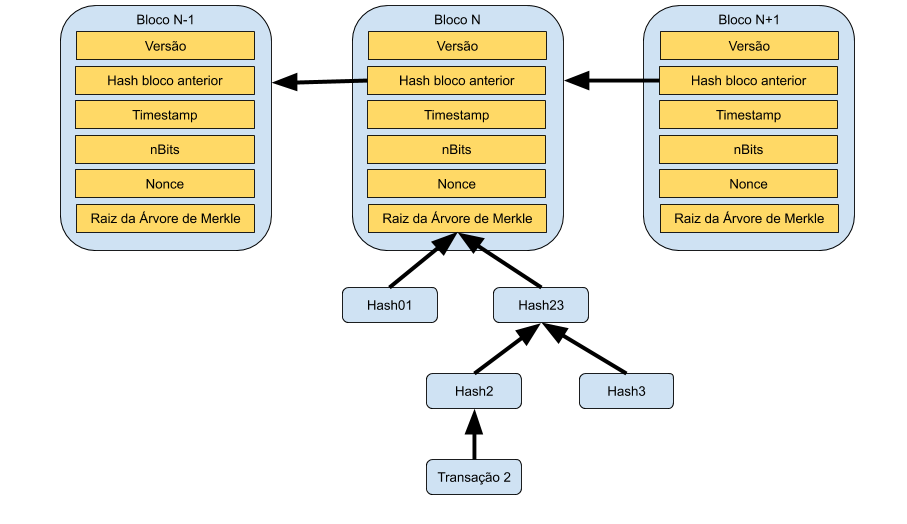
\includegraphics[width=0.9\textwidth]{imagens/esquema_blockchain.png}
\begin{center}
        Fonte: Adaptado de \cite{blockchain:bitcoin_whitepaper} e \cite{blockchain:seguranca_desafios}
\end{center}
\label{fig:esquema_blockchain}
\end{figure}

Na Figura \ref{fig:esquema_blockchain} é mostrada a estrutura do \textit{Blockchain}, como se dá o encadeamento e as características de um bloco individual. 
%
Cada um dos componentes mostrados na parte interior diz respeito a uma variável que porta valores importantes para a construção do bloco, sua identificação e comunicação com a rede.
%
O primeiro campo é a versão do protocolo, e serve basicamente para indicar quais regras de validação devem ser seguidas porque essas podem ser alteradas ou atualizadas com o passar dos anos.
%
O segundo campo compreende o valor de \textit{hash} do bloco anterior e serve, como mencionado anteriormente, para ligar a cadeia. O terceiro campo trata-se do \textit{timestamp} da construção do bloco e por razões óbvias pode levemente variar, uma vez que a assinatura de tempo também é levada em conta no cálculo do \textit{hash} e dessa forma não representará o tempo da finalização do bloco em si.
%
O quarto campo (\textit{nBits}) é responsável por representar o nível de dificuldade de mineração do bloco, ou seja, o quão difícil é gerar um \textit{hash} que seja aceito pela rede. O valor do campo trata-se do número de bits que devem ser iguais a zero no início do \textit{hash} proposto como possível solução para o bloco, caso tal condição seja satisfeita, uma solução válida é encontrada.
%
O quinto campo é o \textit{Nonce} que é um número que começa em zero e após cada \textit{hash} inválido criado é incrementado em um, de modo que se possa tentar gerar um \textit{hash} distinto possivelmente válido para o mesmo conjunto de informações \cite{blockchain:mastering_bitcoin}.

%
O último campo é a raíz da árvore de Merkle que é uma das principais estruturas do \textit{Blockchain}, nela cada nó não final terá o conteúdo igual ao \textit{hash} de seus dois filhos. Assim, nós finais representam algum tipo de dado - nesse caso transações - e os nós ascendentes serão o resultado de sucessivas aplicações da função de \textit{hash} até a raiz, que representa a estrutura como um todo \cite{blockchain:capitulo5}.
%
Por sua vez, a árvore de Merkle é uma estrutura particularmente interessante pois permite o armazenamento parcial dos dados sem comprometer a sua integridade, isso se dá devido à possibilidade de não possuir fisicamente certos ramos, porém estes ainda estarem descritos na estrutura graças ao \textit{hash} de seu pai. Portanto, após a criação da árvore e validação do bloco cujo qual ela pertence um outro usuário da rede não precisa armazenar completamente os dados de todas as transações presentes no bloco para que a cadeia faça sentido, é possível guardar apenas a raiz da árvore ou, no caso de uma verificação pessoal de transações, requisitar à rede que envie um certo ramo específico correspondente a uma transação ou até mesmo grupos de ramos com transações. As vantagens trazidas por tal conceito em relação ao espaço de armazenamento necessário são vastas, principalmente quando confrontadas com a crescente quantidade de blocos nas cadeias e o espaço que ocupam \cite{blockchain:seguranca_desafios, blockchain:bitcoin_whitepaper}.

%
Outra característica importante da tecnologia garantida pelo segundo e último campos é a integridade da cadeia e das informações nela contidas. A existência dos dois campos se complementa pois qualquer tentativa de adulteração em uma das transações, graças às propriedades fundamentais da árvore de Merkle, implicariam em mudança nos \textit{hashes} de todos os nós ascendentes inclusive a raiz, o que influencia na construção do \textit{hash} do bloco como um todo \cite{blockchain:arvore_merkle}.
%
Dessa forma, como o \textit{hash} do bloco anterior é utilizado na criação do bloco atual e o mesmo ocorre para o bloco anterior em relação ao seu predecessor e da mesma forma para todos os blocos ascendentes na cadeia, se qualquer informação sobre as transações for modificada em qualquer um dos blocos predecessores, os \textit{hashes} de todos os consecutivos também serão alterados, o que cria um efeito em cascata que ao atingir o último bloco torna simples a verificação de uma tentativa de adulteração dos dados pela simples comparação dos \textit{hashes} \cite{blockchain:bitcoin_whitepaper}.

\subsection{Formas de redes de \textit{Blockchain}}
\label{subsec:blockchain:pub_priv}

Dentre as redes de \textit{Blockchain} existentes há diferentes modelos de funcionamento para cada uma. Esses modelos dizem respeito principalmente à acessibilidade que os usuários tem para com a cadeia e quanto poder eles têm para operar sobre os registros, no que toca a inserção, visualização e conferência dos dados. Essas formas de funcionamento das redes de \textit{Blockchain} são três \cite{blockchain:formas_redes}:
\begin{itemize}
    \item \textbf{Redes públicas:} Nas redes públicas todos os usuários tem acesso à rede de maneira completa, assim qualquer indivíduo ou entidade pode visualizar o conteúdo que está guardado nos registros e por conta própria averiguar a conclusão ou integridade de repasses transacionais. É possível também que estes, uma vez conectados à rede, possuam fundos e possam efetuar transações para outros usuários, assim como participar dos processos de consenso para validação de blocos. O processo de conexão é dado simplesmente pela obtenção de um endereço válido reconhecido pela rede, geralmente disponibilizado aos participantes através de uma carteira digital que pode ser instalada em uma máquina convencional em poucos passos. Exemplos desse formato de redes são o \textit{Bitcoin} e o \textit{Ethereum}, para os quais existem também diversos sites de terceiros que apresentam informações completas à respeito dessas cadeias de maneira estruturada, como o \textit{Blockcypher} \cite{blockchain:blockcypher} e o \textit{Etherscan} \cite{blockchain:etherscan} respectivamente.
    \item \textbf{Redes Privadas:} Em redes privadas, ao contrário das públicas, somente um grupo seleto de usuários têm acesso aos dados registrados e podem ou não possuir privilégios de execução de transações e participação no processo de consenso. Muitas vezes essas redes pertencem somente a uma empresa central que usa as vantagens do \textit{Blockchain} para auditabilidade e controle dos dados da organização, possuindo um conjunto interno de nós aprovados que podem operar sobre a cadeia. Em tais casos, a participação de usuários externos não é permitida, uma vez que também não há interesse em divulgação de dados sensíveis da empresa que podem estar localizados na cadeia.
    \item\textbf{Redes de consórcio}: Uma rede de consórcio representa um meio termo entre redes públicas e privadas. Nesse modelo o acesso aos dados pode ser público ou restritivo - limitado à quantidade de acessos ou de verificação de informações - enquanto o conjunto de nós que operam sobre a rede é restrito a um grupo confiável que não costuma ser grande como em redes públicas. Esse modelo é utilizado geralmente em aplicações que operam entre negócios, de modo que as instituições controlam a rede no que toca o processo de consenso e transações e usuários públicos podem, em algum nível, ter acesso aos dados da rede. Um exemplo conhecido de rede de consórcio é o \textit{Hyperledger Fabric} \cite{blockchain:hyperledger}.
\end{itemize}

A forma de acesso da rede escolhida para o presente protocolo será levantada na Seção \ref{ch:proposta}.

\subsection{Consenso}
\label{subsec:blockchain:consenso}

Existem diversas formas para obtenção de consenso em redes de \textit{blockchain}, estas independem dos modelos de rede citados na seção \ref{subsec:blockchain:pub_priv} e podem variar de acordo com a necessidade de cada cadeia. A grande diferença nos métodos de consenso reside principalmente na forma de escolha de quem minera o bloco e como esse processo acontecerá.

%
Nas redes públicas de \textit{blockchain} o processo de consenso comumente utilizado é o \textit{Proof of Work}. Os participantes devem provar sua identidade através de um extenso uso computacional para gerar um bloco, o primeiro a conseguir tal objetivo é considerado o criador. Esse algoritmo começa com o \textit{pool} de transações, no qual residem todas as transações efetuadas, porém ainda não confirmadas. Nela os usuários que decidiram participar do processo de mineração escolhem um conjunto de transações, verificam-nas e então constroem uma árvore de Merkle. Ao possuir o \textit{hash} da raiz da árvore o processo de mineração em si pode começar, para tal, o minerador tenta criar um hash que compreende todo o bloco e que respeita o nível de dificuldade imposto pela rede (\textit{nBits}, Seção \ref{subsec:blockchain:specs}), ou seja, que começa com a quantidade de zeros estipulada. Inicialmente o valor do \textit{Nonce} começa zerado e se a primeira tentativa de criar o \textit{hash} não alcança o resultado necessário este deve ser refeito, agora com o valor de \textit{Nonce} incrementado em um e o mesmo acontecerá para cada resultado mal sucedido da função de \textit{hash} \cite{blockchain:capitulo5, blockchain:survey_bitcoin}.
%
Esse processo de tentativas de \textit{hash} é realizado simultaneamente por todos os usuários e como as características referentes ao \textit{timestamp}, transações e ordem das mesmas na árvore provavelmente irá variar entre eles, como resultado emerge uma corrida que possui chances teoricamente iguais para todos os participantes, tendo em vista que por tratar-se de um algoritmo estocástico a solução correta pode tanto ser encontrada na primeira ou na última tentativa executada.

%
Na prática, quanto mais poder computacional um usuário ou grupo de usuários - no caso de uma \textit{mining pool} - possuir (\textit{i.e.} quanto mais rápido se consegue testar as soluções) maiores são as chances de que o bloco seja minerado por tais entidades. Eventualmente o valor do \textit{Nonce} testado por um usuário pode chegar ao seu máximo - no \textit{Bitcoin} são reservados 32 bits para esse campo, o que equivale a cerca de quatro bilhões de possíveis valores não negativos - impossibilitando o minerador de continuar o trabalho. Para resolver esse problema existe outro valor chamado \textit{extraNonce} que reside no nó mais a esquerda da árvore e que deve ser incrementado em uma unidade toda vez que o número de tentativas do \textit{Nonce} original acaba \cite{blockchain:mastering_bitcoin}. 

Em redes que utilizam o \ac{PoW} o valor do campo \textit{nBits} que representa a dificuldade de mineração é aumentado de maneira recorrente dentro de um certo intervalo de tempo. Essa ação é tomada para acompanhar a evolução do hardware, de modo a contrabalancear o poder computacional que aumenta constantemente. Esse processo, entretanto, gera custos energéticos altos, um problema enfrentado em diversas áreas da computação e que representa perdas econômicas e possivelmente ambientais devido às fontes dessa energia. Para contrapor esse obstáculo foram propostas outras formas de consenso menos dispendiosas e prejudiciais.

%
O \ac{PoS} trata-se de uma forma de atingir consenso que baseia-se na quantidade de fundos que os participantes tem daquela moeda, assim usuários mais abastadas terão probabilidades maiores de serem escolhidos para minerar os blocos porque acredita-se que não seria do interesse deles sabotar a rede sobre a qual investiram uma quantidade considerável de recursos. Então para escolher o participante minerador é feito um sorteio ponderado pela porcentagem de patrimônio na rede e o escolhido será o único encarregado do processo de mineração. 
%
O \ac{PBFT} é uma forma de consenso baseada na tolerância de falhas bizantinas e trata-se basicamente de um sistema de votação, comportando até 1/3 de nós maliciosos e necessitando que todos os nós da rede sejam conhecidos. O \ac{DPoS} é uma forma de consenso derivada do \ac{PoS} porém trata-se de uma democracia representativa, ou seja, os detentores de fundos na rede delegam nós para participarem do grupo responsável pelo processo de mineração, diminuindo assim, o tempo necessário para validar os blocos graças ao menor número de participantes envolvidos no processo \cite{blockchain:survey}. 

%
Existem também formas alternativas como: \ac{PoB} na qual os usuários devem gastar ou, como sugerido pelos criadores, "queimar" moedas para receberem chances de minerar um bloco, o que equivaleria ao gasto realizado para comprar \textit{hardware} em redes baseadas no \ac{PoW} porém, graças ao algoritmo empregado, não há necessidade de grande poder computacional para a criação dos blocos \cite{blockchain:PoB}; \ac{PoC} é uma forma de consenso baseada no espaço em disco que um usuário aloca para provar sua identidade \cite{blockchain:origem_PoC} e mais especificamente, no contexto das criptomoedas, um usuário dedica tempo inicial para criar um conjunto de \textit{hashes} que podem servir como solução para os blocos e povoa parte significativa de seu disco com esses dados. No processo de consenso os \textit{hashes} são recuperados da maneira mais rápida possível para tentar minerar o bloco e obter a recompensa \cite{blockchain:burstcoin_PoC}. Existem outras diversas formas menos exploradas de atingir consenso nas redes de blockchain, por exemplo as desenvolvidas para soluções específicas, como é o caso do trabalho de \citeauthor{blockchain:energia_dc} de \citeyear{blockchain:energia_dc} ou ainda outras apenas propostas no meio acadêmico como a \textit{Proof of Luck} \cite{blockchain:PoL}. A forma de consenso escolhida para o presente protocolo será tratada na seção \ref{ch:proposta}.

\subsection{Transações}
\label{subsec:blobkchain:transacaoes}

Para abordar o conceito das transações nas redes de \textit{Blockchain} será utilizada a arquitetura transacional do \textit{Bitcoin}, esta por ser a primeira criptomoeda no mercado e precursora da popularização da tecnologia é tomada como modelo e ponto de partida para a elaboração de novos sistemas desse tipo. Entretanto, a utilização dessa arquitetura não é mandatória e suas características podem e devem ser alteradas para melhor abranger as necessidades do projeto, como no caso do presente protocolo.

%
O modelo de transações do \textit{Bitcoin} funciona como um livro de registro fiscal que possui um conjunto de entradas e saídas para controle de créditos e débitos. Uma transação em si será composta por um conjunto de entradas que apontarão para as saídas de outras transações - encarregadas de assegurar os proventos monetários anteriores - e um conjunto de saídas que serão responsáveis por atribuir o direito de posse desses recursos para um ou mais usuários. Assim, tanto os registros de entrada quanto os de saída representam valores da moeda que, no caso das entradas, devem pertencer ao usuário realizando a transação e no caso das saídas, uma redivisão das entradas para pagamento dos destinatários \cite{blockchain:documentacao_bitcoin}. A Figura \ref{fig:blockchain:transacao} mostra a organização interna de uma transação na rede do \textit{Bitcoin}.

\begin{figure}[ht]
\caption{Esquema de uma transação.}
\centering
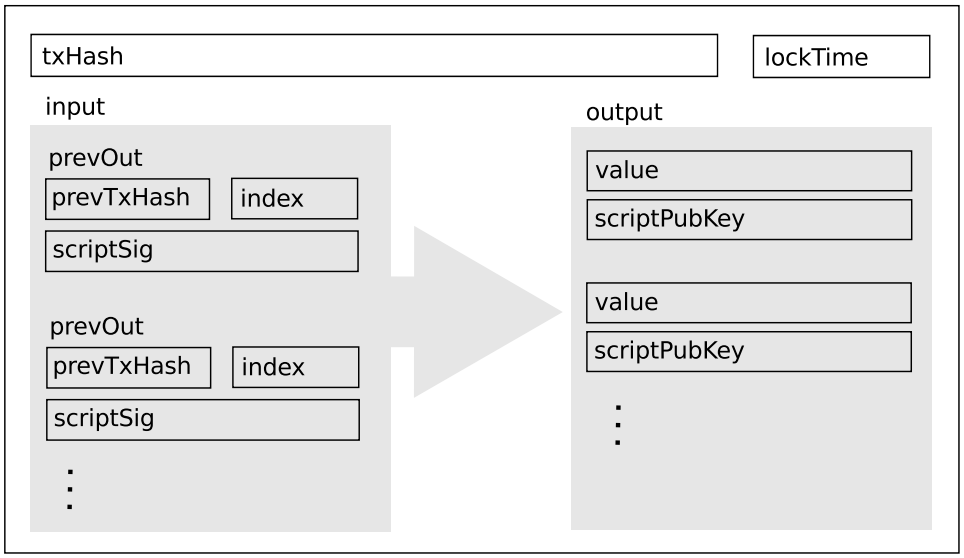
\includegraphics[width=0.75\textwidth]{imagens/esquema_transacao.png}
\begin{center}
        Fonte: Extraído de \cite{blockchain:survey_bitcoin}.
\end{center}
\label{fig:blockchain:transacao}
\end{figure}

A estrutura de uma transação compreende primeiramente o um valor de \textit{hash} para a mesma, responsável por identificá-la na rede. Em seguida há o campo referente ao \textit{locktime} que define quanto tempo - ou quantos blocos confirmados - é necessário esperar antes que as saídas dessa transação possam ser usadas como entrada de uma outra, não sendo um campo obrigatório. A seguir há uma lista não nula de entradas e saídas de transações. Para cada entrada são listados dados referentes ao \textit{hash} da transação anterior e também ao índice da saída dela, cujo valor pode ser utilizado pelo usuário que cria a transação atual, desde que este tenha direito sobre a movimentação do mesmo. Para cada uma das saídas é definido o valor monetário e o \textit{scriptPubKey}, que trabalhará em conjunto com o \textit{scriptSig} das transações que referenciarem essas saídas como insumo. Ambos esses campos são utilizados para a verificação da posse de recursos e cada um deles carrega metade de um \textit{script} da linguagem de programação do \textit{Bitcoin} destinada a esse fim (retomada na Seção \ref{sec:blockchain:smart_contracts}).

%
%
%refazer o parágrafo seguinte, falta clareza
%
%
Quando uma transação deseja utilizar certa saída de outra, é necessário preencher o campo \textit{scriptSig} com a chave pública e uma assinatura que servirá de certificado da chave privada do usuário que reivindica a propriedade. Então, se a execução do \textit{script} contido no \textit{scriptPubKey} da saída, utilizando os parâmetros contidos no \textit{scriptSig} resultarem em uma \texttt{verdade} assume-se que esse usuário é dono das moedas e pode gastá-las. Esse fato pode ser confirmado como verdadeiro porque o usuário que escreve o \textit{script} da saída inclui o endereço de seu destinatário. Então, quando acontece a execução são usadas as duas informações presentes nos parâmetros para construir o endereço público do destinatário e este é comparado com o endereço previamente armazenado na saída. Se a comparação for verdadeira, então a movimentação é aprovada.
%
O conjunto de saídas de transações ainda não gastas de um usuário é chamado de \ac{UTXO} e para que uma nova transação seja aceita é preciso que suas entradas necessariamente referenciem \acp{UTXO}. Os nós que decidem participar dos processos de mineração normalmente mantém um registro dessas transações não utilizadas na memória principal, além do habitual registro em memória secundária. As saídas de transações que já foram referenciadas e que consequentemente tiveram seus fundos utilizados por algum usuário são chamadas de \ac{STXO} - saídas de transação gastas - e dessa forma não podem mais ser referenciadas por nenhuma nova transação e, caso essas tentem, reprovarão no processo de validação.
%
A conexão de entradas e saídas de transações gera diversos fluxos para as moedas e estes eventualmente devem começar em algum lugar. O ponto de partida de um fluxo de transações é sempre uma transação especial que insere novos \textit{Bitcoins} na rede quando um bloco é minerado, essa transação é chamada de \textit{coinbase transaction} e não possui nenhuma entrada de outras transações. O valor da recompensa dessas transações no começo da rede equivalia a 50 \textit{Bitcoins} e é reduzido pela metade, desde então, a cada 210.000 blocos validados. Outra peculiaridade é o tempo de espera, são necessários ao menos 100 blocos confirmados para que uma \textit{coinbase transaction} possa ser gasta \cite{blockchain:survey_bitcoin}.

%
Um outro tipo de recompensa dada para o usuário que minera o bloco é um valor chamado \textit{transaction fee} que, como o nome sugere, trata-se de uma taxa que é paga ao usuário que minera o bloco vindo da diferença entre as entradas e as saídas das transações. Para tal, o valor total das entradas deve, obrigatoriamente, ser maior ou igual ao valor total das saídas de modo que a existência dessa taxa seja possível.

Para o protocolo proposto, as transações podem assumir diferentes formas e representar objetivos de transferência diferentes, esses conceitos serão apresentados na Seção \ref{ch:proposta}.

\subsection{Carteira digital e cliente do usuário}

Para que um usuário tenha acesso a uma rede  de \textit{Blockchain} é necessário que ele possua um endereço nessa rede que seja reconhecido por todos os participantes e que seja passível de verificação no caso da realização de transferências. Tal endereço consiste unicamente de um par de chaves privada e pública, sendo a primeira um número aleatório de 256 bits e a segunda o resultado do uso da primeira como parâmetro de multiplicação no modelo de criptografia \ac{ECDSA}. A chave privada é costumeiramente gerada através de uma carteira digital, que também é responsável por armazenar esses dados - pois em caso de perda da chave privada, o conjunto de moedas guardado pela respectiva chave pública também se perde - para o uso, possíveis migrações para outro dispositivo ou mudança de conta. Aconselha-se aos usuário que troquem seu conjunto de chaves periodicamente, preferivelmente a cada nova transação, de modo a evitar possíveis ataques de descoberta de identidade ou comparação de chaves públicas. Para tal fim, há um histórico de desenvolvimento de modelos de carteiras que que gerem múltiplas chaves. Nos primórdios eram usadas carteiras randômicas, que geravam aleatoriamente um conjunto de n chaves privadas, sendo que todas deveriam ser armazenadas para a possibilidade de migração. O segundo modelo foram as carteiras determinísticas, que geravam uma primeira chave aleatória e posteriormente criavam novas a partir dela, sendo preciso apenas armazenar o dado inicial para que fosse possível refazer todo o processo de computação da criação das chaves posteriores. O terceiro modelo e mais usado atualmente são as carteiras determinísticas hierárquicas, que assemelham-se as suas predecessoras na geração de um dado inicial e reconstrução das gerações, porém gera novas chaves em uma estrutura de árvore, que possui certas vantagens principalmente nos âmbitos da quantidade de chaves diversas que podem ser geradas e no compartilhamento das mesmas (\textit{e.g.} no caso de diferentes endereços sob o domínio de uma mesma entidade ou empresa, destinados a possíveis departamentos ou funcionários).

%
Outro papel fundamental da carteira é agir como cliente para o usuário e atuar como ponto de entrada na rede, no qual muitas tarefas importantes são abstraídas. Nelas, a criação de novas transações se apresenta através de uma interface gráfica para o usuário, o que facilita a escrita e o entendimento, diminuindo a probabilidade de ocorrência de erros. As chaves muitas vezes são mostradas também de maneira formatada, através do uso de mnemônicos, simplificando o processo de armazenamento em meios não necessariamente digitais. Outras funções de nível mais baixo como mensagens de aviso e requisição para outros nós, bem como a escolha das saídas de transações disponíveis para serem utilizadas como entradas para novas transferências são todas tarefas administradas pelas carteiras.

%
Existem ainda, diversas implementações de carteiras independentes e com diferentes funcionalidades quando comparadas às opções nativas ou padrão da rede. Essas também voltam-se para diferentes dispositivos e plataformas, expandindo o poder de escolha e personalização dos usuários na maneira de se relacionar com a rede. Por fim, muitas \textit{Blockchains} fornecem também bibliotecas para o desenvolvimento de novas carteiras, de modo que empresas ou até usuários criem soluções que se adéquem perfeitamente às suas necessidades.


\section{Contratos inteligentes}
\label{sec:blockchain:smart_contracts}

Contratos inteligentes são um conceito que precede o surgimento das criptomoedas e que define uma espécie de regulamentação digital responsável por registrar regras que as partes envolvidas em um acordo legal devem cumprir, estabelecendo punições específicas para diferentes formas de infrações legais. Um contrato inteligente é autônomo na execução e consequentemente na imposição das normas contratuais sobre os envolvidos, representando uma abstração virtual de contratos legais firmados no mundo real \cite{smart_contracts:szabo}. Um exemplo interessante, também proposto por  \citeauthor{smart_contracts:szabo} em \citeyear{smart_contracts:szabo}, é o de um contrato inteligente que regulamentaria a segurança no uso de um veículo. Nesse contrato, algum tipo de imposição física limitaria o uso do automóvel somente ao proprietário, graças à confirmação de uma chave digital criptográfica e se qualquer usuário que não o dono - ou conjunto de donos - tentasse utilizar o veículo, este não obteria êxito. Se por algum motivo esse veículo estivesse alienado como garantia à uma forma de empréstimo, o não pagamento das parcelas ou até mesmo a morte do dono acarretaria na execução do contrato e na transferência automática do direito de posse e utilização do bem ao banco ou instituição responsável pelo empréstimo, sendo tomadas as devidas precauções para não realizar o descrédito da posse em situações críticas (\textit{e.g.} o usuário está utilizando o veículo). Dessa forma, houve uma punição imposta pelo contrato ao usuário em débito, representada pela remoção de seu direito de posse e transferência para a entidade credora. Torna-se portanto simples o entendimento das obrigações das partes, manutenção de rotinas e as punições desferidas sobre os infratores do contrato.

%
No contexto das criptomoedas especificamente, um contrato inteligente possui as mesmas características da definição geral, porém opera exclusivamente sobre transações e movimentação de dados transacionais, servindo como maneira de executar operações mais complexas divisão e retenção de fundos, por exemplo \cite{blockchain:mastering_bitcoin}. Quando ocorre a invocação de um contrato inteligente, no caso da máquina de estados distribuída que é a rede de \textit{blockchain}, este deve ser executado por todos os participantes para garantir a consistência dos registros em todas as cópias da cadeia. Da mesma forma que o modelo transacional, diferentes redes implementam diferentes formas de contratos inteligentes, ou até não os implementam de forma alguma. O Hyperledger Fabric, que trata-se de um \textit{framework} para o desenvolvimento de \textit{blockchains} privadas ou de consórcio, voltadas para comunicação entre diferentes companhias utiliza um modelo de \ac{SC} que além das definições básicas ainda implementa conceitos relativos ao seu meio específico. Características relacionadas a modelos de negócio, \textit{chaincodes} para agrupar contratos baseando-se em grupos de execução para fins semelhantes, políticas de responsabilidade de empresas sobre as transações geradas por \ac{SC} entre outras são modelos únicos implementados por esse \textit{framework} \cite{smart_contracts:hyperledger_fabric}. As criptomoedas mais populares, \textit{Bitcoin} e \textit{Ethereum}, possuem versões menos focadas em nichos específicos do mercado, representando em seus contratos apenas transferências de moedas, cada implementação tendo suas peculiaridades que acarretam em vantagens ou desvantagens em relação a certos aspectos.

\subsection{Contratos no \textit{Bitcoin}}

Na rede do \textit{Bitcoin}, que novamente por ser a primeira criptomoeda funcional introduziu o conceito desse modelo, os contratos são implementados por meio da linguagem \textit{Script} (mencionada na Seção \ref{subsec:blobkchain:transacaoes}) que tem sua utilização fundamentada na verificação de propriedade de fundos monetários que pode ser feita de diversas formas. Essa linguagem é bastante simples - quando comparada as linguagens de alto nível que circulam pelo mercado nos dias presentes - e baseia-se em uma pilha para armazenamento das informações, podendo resolver todas as classes de problemas que um autômato finito com pilha satisfaz. Essa característica foi propositalmente definida como uma escolha de arquitetura por razões de segurança e consistência da cadeia, porque uma vez operando sobre um ambiente distribuído e não necessariamente confiável há necessidade de que seja possível prever o estado da execução de um contrato e que o mesmo seja coerente e alcançável por um conjunto amplo de usuários e possivelmente diverso em \textit{hardware}. A \textit{Script} funciona através de operações que adicionam e retiram dados da pilha e operam sobre esses até que essa encontre-se vazia, assim é possível criar programas que embora simples, realizam com perfeição as necessidades da rede. Os \textit{scripts} são escritos de maneira personalizada e adicionados no campo \textit{scriptPubKey} de cada saída, sendo executados mediante a conferência da validade de uma transação e utilizando como parâmetro o \textit{script} que é armazenado no campo \textit{scriptSig} da transação que a consome \cite{blockchain:documentacao_bitcoin}.

%
Existe um conjunto de \textit{scripts} padrão que realizam ações recorrentemente necessitadas por usuários e que atendem a objetivos diferentes. Transações que utilizam formas verificação do conjunto de \textit{scripts} padrão tem a certeza de que não serão negligenciadas por potenciais mineradores. \textit{Scripts} personalizados, entretanto, podem facilmente fazer com que suas transações não sejam tomadas como participantes em blocos candidatos para mineração \cite{blockchain:mastering_bitcoin}. \textit{Scripts} padrão são responsáveis por diferentes formas de verificação e dentre estas estão: 
\begin{itemize}
    \item \textbf{Pay-to-Pub-Key-Hash (P2KH):} é tratado como se fosse o algoritmo padrão para a verificação de posse e quando é executado simplesmente confere se a assinatura e chave pública fornecidas no \textit{scriptSig}, ao serem submetidas à função de \textit{hash}, geram o endereço correspondente ao escrito no script de trava da saída.
    %
    \item \textbf{Pay-to-Multisig (P2MS):} Esse \textit{script} é utilizado para travar uma transação com um conjunto de $n$ chaves públicas, de modo que seja necessário um subconjunto $m$ de assinaturas para liberar a utilização dos recursos por parte de uma transação \cite{blockchain:mastering_bitcoin}. Um exemplo de uma possível utilização desse script seria o conceito de contas conjuntas, onde é necessária a aprovação de todos os titulares para que se possa mover fundos da conta para terceiros.
    %
    \item \textbf{Pay-to-Script-Hash (P2SH):} Através dessa forma padronizada torna-se possível que um usuário A transfira recursos para um usuário B e que embora o primeiro seja responsável por escrever a transação, o \textit{script} de travamento seja escrito por B. Como é B quem deve realizar o destravamento não há nenhum problema em tal modelo e podem haver situações em que seja coerente, do ponto de vista de B, a existência de algoritmos mais complexos ou completos para a liberação das moedas \cite{smart_contracts:learn_me_a_bitcoin}.
    % O funcionamento, dessa forma, começa com B enviando o hash do \textit{script} que deseja no travamento para o usuário A. Esse então, simplesmente adiciona-o ao \textit{scriptPubKey} com outras operações de verificação e movimentação da pilha embutidas com o único propósito de comparação com o script de destravamento para que, obviamente, não hajam adulterações no resultado esperado. Quando o usuário B deseja usar a transação ele povoa o \textit{scriptSig} com o script que ele enviou ao usuário A junto aos parâmetros necessários para a sua execução. Esse algoritmo é então adicionado à pilha e uma cópia desta é feita. O scriptPubKey é então executado criando uma
    \item \textbf{OP\_RETURN:} Essa operação padronizada é relativamente recente e foi adicionada ao protocolo no ano de 2014 \cite{smart_contracts:bitcoin_0.9} e tem como principal objetivo fomentar a possibilidade do armazenamento de dados não relacionados à transações monetárias na cadeia, tópico que até então gerava discussões desde que o momento em que certos usuários criaram transações substituindo o \textit{scriptPubKey} por dados não relacionados ao modelo, como imagens ou \textit{hashes} de documentos para comprovação de existência. Tal prática criava transações "fantasma" na cadeia que nunca poderiam ser gastas por conter um \textit{script} inválido \cite{blockchain:mastering_bitcoin}. No modelo atual quando uma transação atribui ao algoritmo de travamento a opção \textbf{OP\_RETURN} esta não pode mais ser utilizada como \textit{input} de nenhuma outra e dessa forma, quaisquer valores que foram adicionados à transação são perdidos. O restante do espaço que anteriormente seria destinado para parâmetros e operações do \textit{script} destina-se para armazenamento de dados brutos que não possuem significado ou são interpretados pelo protocolo \cite{smart_contracts:learn_me_a_bitcoin}. É importante ressaltar, entretanto, que não é recomendado o armazenamento de informações não relacionadas à moeda na cadeia do \textit{Bitcoin} por forçar o armazenamento desnecessário de arquivos não importantes para a rede  \cite{smart_contracts:bitcoin_0.9}.
\end{itemize}

Há também uma versão mais simples e anterior ao P2PKH que é o P2PK, que por ser um tanto quanto primitiva em comparação com sua sucessora não foi abordada em detalhes. No que toca os algoritmos padronizados para as transações no \textit{Bitcoin} há possibilidade de inclusão de novas formas a cada atualização, o que diversifica as possibilidades de utilização da rede e dos casos do mundo financeiro que ela pode atender. 

\subsection{Contratos no \textit{Ethereum}}

O \textit{Ethereum} foi a rede que oficialmente introduziu ao mundo o conceito de contratos inteligentes como é conhecido hoje, ou seja, contratos que podem representar uma gama quase ilimitada de possíveis situações de movimentação financeira. O grande fator responsável pelas possibilidades de utilização do \textit{Ethereum} é que seus contratos inteligentes são desenvolvidos em linguagens Turing-Completas, dessa forma podendo resolver qualquer problema que uma Máquina de Turing consegue, representando um poder computacional muito maior do que a linguagem \textit{Script} do \textit{Bitcoin} \cite{blockchain:capitulo5}.

%
Embora o Ethereum seja reconhecido principalmente por sua rede de criptomoedas a proposta formal do mesmo é ser uma máquina de estados transacional de fins genéricos. A própria arquitetura da cadeia do \textit{Ethereum} é bastante diferente do \textit{Bitcoin}, tomando como base um modelo de "balanço de contas" e transações sequenciadas, em oposição ao modelo de "transações não gastas (\ac{UTXO})" usado para especificar o estado de um usuário no \textit{Bitcoin}. Outro fator de diferença entre as duas redes é a forma como elas lidam com os endereços ou contas, sendo que no \textit{Bitcoin} apenas usuários possuem endereços e dessa forma, apenas usuários podem ser referenciados como destino de transações. No \textit{Ethereum} há dois tipos de contas: as \acp{EOA} são contas pertencentes a usuários e, portanto, possuem um par de chaves pública e privada e tem a capacidade de criar transações e movimentar fundos através delas, bem como invocar contratos. As \textit{contract accounts} são contas que não possuem chaves privadas e não pertencem a nenhum usuário, existindo apenas para dar sustento aos códigos de contratos inteligentes. Essas contas também possuem a habilidade de realizar transações de moedas. Quando um usuário deseja executar um contrato inteligente na rede do Ethereum, é necessário que ele referencie uma \textit{contract account} como destinatária. Isso fará com que o contrato seja executado como especificado na transação - pois há campos destinados apenas a transmissão de dados e parâmetros para execução de contratos - pela \ac{EVM} \cite{blockchain:mastering_ethereum}.

%
A \ac{EVM} trata-se de uma máquina virtual que possui o intuito de abstrair um ambiente de execução alheio ao \textit{hardware} para o processamento dos \textit{bytecodes} referentes ao código do contrato compilado. Com a chamada de um contrato, todos os usuários que validarem a sua execução invariavelmente executarão o código na \ac{EVM}, esta possuindo um conjunto de estruturas para armazenamento de memória temporária e permanente para contribuir com o estabelecimento do consenso global.
%
Ao que toca os contratos, por serem Turing-completos, não é possível prever o estado final de dada execução nem mesmo os caminhos que serão tomados para alcançar tal estado. 
%
Portanto, usuários diferentes poderiam executar com sucesso um mesmo contrato com números completamente diferentes de iterações e possíveis saídas distintas.
%
No contexto de ambientes confiáveis distribuídos, essa característica pode tornar-se um empecilho por possibilitar a existência de conjuntos de dados distintos em pontos diferentes da rede.
%
Para contornar esse problema o \textit{Ethereum} faz uso de um conceito chamado \textit{gasLimit}, que é responsável por determinar a quantidade máxima de iterações que poderão ser executadas na computação de uma transação ou contrato pelos usuários na \ac{EVM}.
%
Cada tipo de instrução na linguagem possui um custo diferente em \textit{Gas} e na criação da transação deve ser especificado também um campo denominado \textit{gasPrice}, que compreende o preço que o usuário responsável pela transação está disposto a pagar por cada unidade de \textit{Gas} utilizada em seu processamento. Se eventualmente a quantidade de \textit{Gas} acaba o processamento é interrompido e o estado da execução naquele momento é considerado o final. Se a computação não usou toda a quantidade delimitada no \textit{gasLimit} o valor que sobra é ressarcido ao criador, ao passo que os valores utilizados são pagos ao nó que minerar a transação. Assim, quanto maior o \textit{gasPrice} definido na transação, maiores são as chances de que essa transação seja incluída em um bloco, já que uma quantidade maior de mineradores irá incluí-la no bloco que tentam minerar \cite{blockchain:ethereum}.

Todos os dados apresentados neste capítulo servem como base e fonte de estudo para o desenvolvimento e justificativa das escolhas para a presente proposta, apresentada no Capítulo \ref{ch:proposta}.
	\chapter{Proposta}
\label{ch:proposta}

Este capítulo destina-se a explanar a proposta para o problema apresentado. De antemão são apresentadas as escolhas de arquitetura realizadas, referente aos tópicos levantados na Seção \ref{ch:fundamentos}, as justificativas a respeito de cada escolha são explanadas na Seção \ref{}. 

%
\section{Atores participantes}

Os atores que fazem parte da execução do protocolo são, primeiramente os clientes, que entram na rede em busca da escolha de um provedor que atenda aos seus padrões de preço e reputação para realizar a alocação de microsserviços. Seus poderes envolvem o pedido devidamente organizado de uma alocação para a rede, a confirmação de propostas de provedores, prolongação de requisições, convocações de votação para possíveis quebras de contrato e o voto em convocações de outros usuários contra o seu provedor. O segundo grupo de participantes são os provedores, que adentram a rede em busca de novos clientes. Seus poderes envolvem responder a pedidos de alocação com propostas para um ou mais microsserviços distintos e votar em convocações para outros provedores. O terceiro grupo de participantes são os agregadores, que possuem todos os poderes de cliente e provedor mesclados, salvaguardando as requisições de serviço que são puramente para \acp{IaaS} genéricos, não sendo relacionadas a um conjunto de microsserviços como é o caso das requisições dos clientes. 

\section{Definições iniciais da rede}
\label{sec:proposta:definicoes}

O modelo da rede de \textit{Blockchain} escolhido assemelha-se ao do \textit{Bitcoin}, ou seja, fundamentalmente baseada em transações e que utiliza as informações dessas para levantar a situação atual do usuário.
%
A rede proposta, entretanto, não tem seu fim em transações monetárias, assim não trata-se de uma criptomoeda em essência, porém utiliza certas características normalmente adotadas nelas em conjunto com propriedades destoantes que melhor refletem as necessidades do problema abordado.

%
A maioria das informações que transitam entre usuários e que consequentemente são escritas na cadeia se referem puramente a dados de definição e concretização de contratos, desenvolvidas para otimizar e facilitar o processo de contratação de infraestruturas, bem como para possível avaliação posterior.
%
Apenas uma pequena parcela do total de transações conterá movimentação de valores propriamente ditos e estes não servirão como moeda de troca mas sim como medidor da reputação dos participantes. Quanto maior for o montante desse valor possuído por um usuário - referidos a partir do presente momento como pontos de reputação - naturalmente melhor será sua reputação. Esse valor será obrigatoriamente público - característica que novamente destoa das criptomoedas apresentadas no Capítulo \ref{ch:fundamentos} - tanto para os participantes da rede quanto para indivíduos externos. Essa propriedade é definida dessa maneira para atender a um dos objetivos do protocolo que é auxiliar clientes na escolha de provedores de serviço, no qual a reputação é um fator importante. Partindo de tais fatos e complementando a definição da Seção \ref{subsec:blockchain:pub_priv}, a proposta trata-se de uma rede de consórcio, pois apenas um grupo aprovado de usuários pode operar sobre a cadeia, na qual a entrada está sujeita à apresentação de provas de identidade para provedores e agregadores, de modo a garantir a integridade dos processos que nela acontecem. A pesquisa e visualização dos dados na \textit{Blockchain} é pública, logo até usuários que não possuem nenhuma correlação com o sistema podem visualizar dados de transações e de reputação.

%
Na rede os usuários possuem endereços individuais, responsáveis por identificá-los em meio aos outros participantes e possuem também um endereço de grupo, que identifica qual é o tipo daquele usuário. A segunda característica é importante pois como grande parte das transações trata-se de publicação de informações, torna-se interessante que mais de um usuário possa referenciar certos tipos de transação para diversos fins apresentados nas Seções \ref{sec:proposta:fase_contratual} e \ref{sec:proposta:fase_auditoria}.

%
Da mesma forma que no mundo real, não é possível vender ou transferir reputação de uma pessoa ou organização para outra, tal característica também poderá ser observada na rede, portanto um usuário não pode deliberadamente criar uma transação para transferir pontos de reputação. Contudo, a movimentação de tais pontos de fato acontece, embora a parte majoritária das decisões a respeito dessas transferências não caibam ao usuário, mas sim ao protocolo em si e ao processamento distribuído, fato elucidado na Seção \ref{sec:cenario_execucao}. No que toca a execução distribuída no contexto de \textit{Blockchain}, uma grande personagem no processo é a carteira digital ou, de forma mais genérica, o cliente de acesso à rede. Na rede proposta a carteira terá um papel significativo pois além de ser responsável por administrar as chaves, gerar endereços e validar transações e blocos, ainda terá a responsabilidade de julgar quando houve quebra de contrato, também administrando módulos remotos encarregados do processo de monitoração, conceito retomado na Seção \ref{sec:cenario_execucao}.

%
Ao retomar as formas de consenso exploradas na Seção \ref{subsec:blockchain:consenso} conclui-se que o uso de \ac{PoW} convencional não é adequado para tal cenário, porque como agregadores e especialmente provedores podem alocar poderes computacionais elevados para mineração, quando comparados aos usuários, a parte majoritária das minerações seriam de autoria de provedores e agregadores, com apenas aparições esparsas de blocos criados por usuários comuns. Um ambiente como esse, além de injusto com usuários menos favorecidos computacionalmente, implica em uma grande carga de responsabilidade e confiança em um grupo relativamente pequeno de usuários. Esses, mesmo possuindo um histórico possivelmente idôneo também podem vir a praticar ações fraudulentas, de forma que não é possível garantir que manterão o comportamento correto no decorrer da criação dos blocos futuros.

\section{Cenário de execução}
\label{sec:cenario_execucao}

Essa seção tem por objetivo elencar o cenário de execução principal da proposta, assim como características iniciais relativas à estrutura das trocas de mensagens, ordem das mesmas e a relação dos atores com a cadeia e uns para com os outros.

%
O cerne do protocolo, como apontado na Seção \ref{ch:intro} reside na elaboração e verificação de contratos. Para o primeiro passo utiliza-se a cadeia de blocos como forma de comunicação assíncrona e meio de sedimentação das negociações ao longo do tempo. Para a segunda parte, decorrentes de suspeitas de violações de contrato, são convocadas votações a respeito da ocorrência ou não de quebra. Estas são respaldadas por dados de monitoração obtidos por usuários e agregadores que possuem algum tipo de relação contratual de \ac{IaaS} para com o agregador ou provedor sendo acusado, mas também por provedores e agregadores que embora não possuam contratos monitoram seus concorrentes secretamente.

%
As escritas na cadeia - referidas também como transações - quando não assumem o caráter de transferência de pontos de reputação podem ser entendidas como uma publicação e sedimentação de informações, sendo que essas podem ser referenciadas pelos participantes para a realização de novos conjuntos de transações, que resultam na sedimentação de mais informações e assim por diante. Todas essas informações escritas na rede relacionam-se de alguma forma com a elaboração dos contratos e servem basicamente como veículo de comunicação e forma de estabelecer e armazenar os contratos em si. 
%
As transações voltadas para a transferência de pontos de reputação acontecem no estabelecimento de um novo contrato, pois o agregador ou provedor que prestará o serviço ou parte dele tem sua reputação verificada pelo usuário contratante e após a confirmação do contrato entende-se que o usuário confia naquele prestador de serviço. Assim, olhando de forma pragmática, a reputação de um provedor ou agregador é dada pela quantidade de clientes satisfeitos que eles possuem e assume-se que um cliente que acaba de iniciar um contrato está satisfeito, tendo em vista que perante análise inicial as condições do contrato são de seu interesse e não foram violadas.
%
De forma análoga, um provedor ou agregador perderá pontos de reputação quando for declarado culpado de quebra de contrato mediante uma acusação relacionada. Pontos de reputação podem ainda ficar em custódia temporária durante processos de votação, onde é possível que participantes terceiros ganhem ou percam reputação de acordo com a contribuição de dados assertivos ou não, discussão que é retomada na Seção \ref{sec:proposta:fase_auditoria}. 
%
Relativamente, a monitoração entre provedores e agregadores responsável por gerar os dados para votações, não depende necessariamente de nenhum contrato, ou seja, assim que um novo provedor entra na rede ele pode começar a ser monitorado e da mesma forma monitorar seus concorrentes.

%
Para auxiliar a formação do cenário de execução hipotético nas Seções \ref{sec:proposta:fase_contratual} e \ref{sec:proposta:fase_auditoria} é utilizada a figura \ref{fig:cenario_execucao} que trata todas as nuances do processo, envolvendo desde a requisição de serviço até o veredito de violação.

\begin{figure}[h!]
\caption{Cenário de execução completo}
\centering
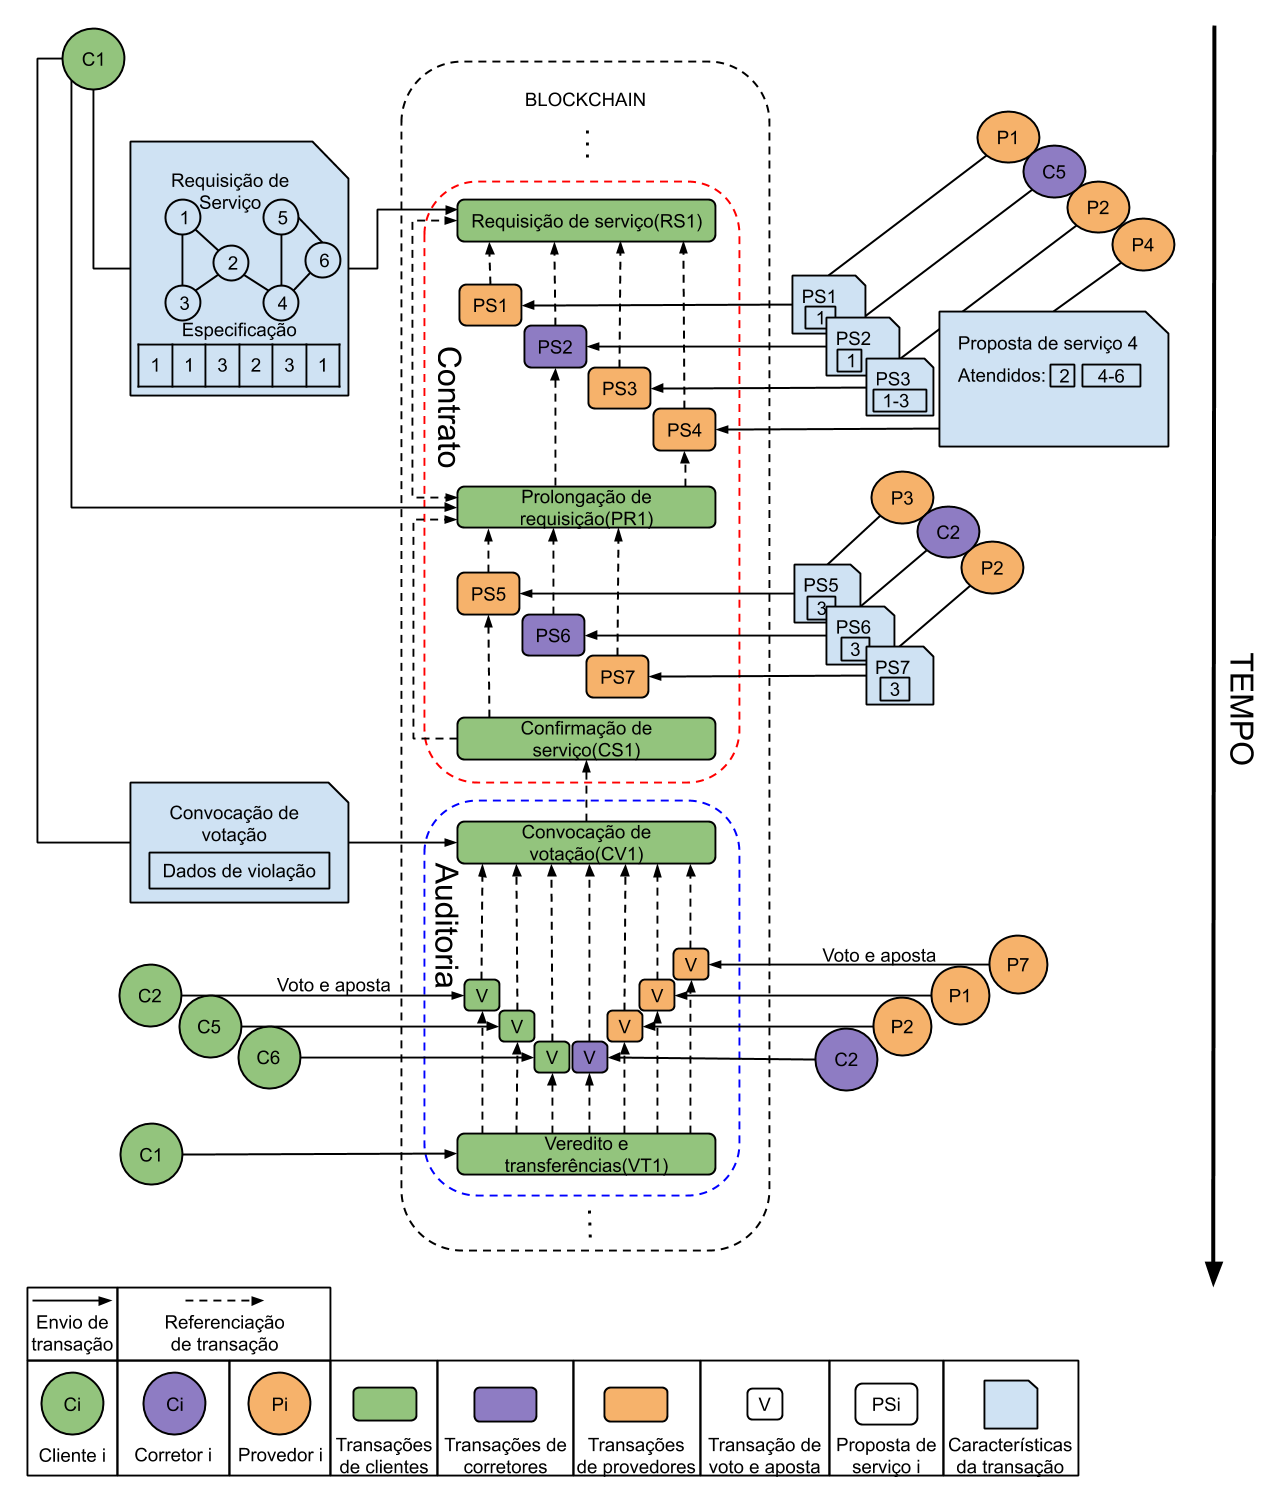
\includegraphics[width=0.96\textwidth]{imagens/cenario_execucao.png}
\begin{center}
        Fonte: Autor
\end{center}
\label{fig:cenario_execucao}
\end{figure}


Assim, clientes envolvidos no processo são representados por círculos verdes e por uma legenda contendo a letra maiúscula C, bem como um índice numérico referente ao cliente em questão. O mesmo vale para provedores e agregadores, que além de serem reconhecidos pelos índices individuais, são representados por círculos laranjas e pela letra P, no caso dos provedores e círculos roxos e pela letra A, no caso dos agregadores. A cadeia de blocos é representada por um retângulo tracejado e referenciações para transações passadas são identificadas através de flechas tracejadas em direção à transação pai. Envios de transações para a rede por parte dos atores são representados por flechas contínuas que iniciam no ator e terminam dentro da \textit{Blockchain}. Detalhes importantes das transações enviadas são mostrados através de retângulos azuis no meio das flechas de envio. Transações de autoria de usuários na cadeia são coloridas de acordo com a cor referente ao tipo do mesmo. Outras Informações específicas a respeito da estrutura das transações e funcionamento de baixo nível do sistema serão explicadas na Seção \ref{}.

\section{Fase contratual}
\label{sec:proposta:fase_contratual}

A fase contratual representa o início de um ciclo completo do protocolo e compreende todo o processo relativo ao estabelecimento de um contrato e as negociações realizadas para tal. Essa fase é representada na Figura \ref{fig:cenario_execucao} por um retângulo tracejado vermelho com a legenda "Contrato".


\subsection{Requisições de serviço}
\label{subsec:proposta:contratual:rs}
%
Os contratos na rede proposta devem ser atômicos, assim não é possível fechar um contrato sem que todos os microsserviços elencados pelo cliente sejam devidamente supridos pela infraestrutura de algum provedor ou agregador. Após a entrada de um usuário na rede este já está apto a estabelecer contratos com provedores, o primeiro passo para realizar esse processo é a escrita de uma nova transação, que representa uma requisição de serviço. Essa requisição de serviço descrevem um conjunto de microsserviços que, como pode ser observado na figura \ref{fig:cenario_execucao}, são organizados em um grafo não direcionado, de forma que os nós representam os microsserviços em si e as arestas os enlaces necessários para que a comunicação seja realizada corretamente. Junto ao grafo encontra-se um vetor com tamanho igual à quantidade de microsserviços, cujo valor de cada célula $i$ representa a infraestrutura requerida para o microsserviço $i$. Por fim, há uma quantidade finita de requisições de serviço abertas que um usuário pode ter em um determinado momento, de modo que quando esse limite é atingido é necessário fechar contratos - se todos os microsserviços foram atendidos com infraestruturas correspondentes - ou finalizá-las para que a criação de novas requisições seja liberada.

\subsection{Definições de infraestrutura}
\label{subsec:proposta:contratual:di}
%
Diferentes microsserviços de uma mesma requisição podem ter necessidades diferentes de infraestrutura e portanto as transações de \ac{RS} devem referenciar outras transações chamadas \ac{DI}, que podem ou não ser escritas pelo usuário que faz a requisição. Na rede, qualquer participante pode escrever um número finito de transações de \ac{DI} e estas podem ser referenciadas por qualquer outro usuário que deseja fazer uma requisição. Assim sendo, provedores podem publicar definições padrão que costumam oferecer, como se fossem planos predefinidos de serviço, enquanto usuários podem criar novas definições para microsserviços com necessidades específicas que podem, eventualmente, servir para outros usuários em condições semelhantes. Atualizações nas definições podem ser feitas pelos criadores em caso da necessidade de adaptação de infraestruturas para novos contratos, sendo representadas por uma nova \ac{DI} que referencia a anterior. \acp{DI} apenas podem ser atualizadas caso já exista algum contrato firmado que as referenciem, para evitar o surgimento de definições órfãs ou o superpovoamento de definições pelos usuários. Portanto, usuários podem ter até $n$ definições existentes sem referenciação e nada impede o criador ou outros clientes de referenciar versões passadas de uma \ac{DI}.

%
O objetivo dessa escolha de arquitetura é primeiramente reduzir a duplicação de informação, uma vez que muitos clientes podem querer utilizar arquiteturas idênticas, cujas diferentes requisições de serviço não precisam reter as informações consigo, mas apenas referenciá-las. Consequentemente, as dificuldades de escalabilidade da rede se tornam mais brandas, devido ao menor volume de dados que é precisa armazenar em todos os dispositivos conectados. Esse tipo de abordagem leva à consequente formação de uma "biblioteca" pública de definições de infraestrutura, na qual usuários publicam informações e utilizam as de terceiros.

%
\subsection{Propostas de serviço}
\label{subsec:proposta:contratual:PS}

Após a escrita de uma \ac{RS} na cadeia, propostas de serviço podem ser enviadas para suprir tal demanda. \acp{RS} são escritas de modo que a saída da transação seja travada não para o endereço de um usuário, mas sim para endereços do grupo de agregadores e para o grupo de provedores. Esses podem referenciar a requisição em questão criando novas transações chamadas \ac{PS}, que contém uma oferta da infraestrutura desejada para um ou mais microsserviços. Uma informação importante contida em tal forma de transação é o preço que o provedor se dispõem a realizar o serviço descrito na proposta, uma vez que grande parte das informações a respeito da alocação em si já foram definidas na \ac{DI} referenciada pela requisição.

\subsection{Prolongação de requisição}
\label{subsec:proposta:contratual:pr}
%
Um cliente, após abrir uma requisição, pode esperar por tempo indeterminado propostas de serviço até encontrar as que mais se adéquem às suas preferências. Ocasionalmente, o aparecimento de novas propostas para uma requisição cessa, decorrente do envelhecimento da transação em questão na cadeia, que acarreta em baixa visibilidade para outros provedores. Outro possível cenário trata-se do cliente se interessar por propostas que contemplam uma parcela dos microsserviços, mas não por aquelas que contemplam outra, da mesma forma que a requisição pode não receber propostas suficientes para abranger os microsserviços em completude. Na ocorrência de tais casos, o usuário pode criar uma \ac{PR} que serve para explicitar quais das propostas feitas até o momento foram escolhidas para a requisição, sendo indicadas através da referenciação das transações das \acp{PS}. Após a criação dessa transação, o efeito gerado na rede é o reavivamento da requisição, que acontece devido a transmissão da \ac{PR} como uma nova transação, atraindo o olhar de provedores e agregadores. Na prolongação deve ser registrado, além das propostas aceitas, quais microsserviços não foram atendidos, de modo a agilizar o processo posterior de verificação dessas transações, para que não seja necessário vasculhar a cadeia toda para encontrar a requisição e obter tais dados.
%
Novas \ac{PS} podem então ser feitas por parte dos prestadores de serviço, agora referenciando não a requisição original, mas sim a prolongação de requisição relacionada, buscando assim finalizar o processo de escolha dos serviços. A quantidade de \ac{PR} que uma requisição pode ter é limitada, pois pode ocorrer de que certos microsserviços apenas não sejam mercadologicamente viáveis para o atendimento dos prestadores. Em face de tal ocorrido, a única alternativa é recomeçar o processo criando uma requisição em que as características dos microsserviços não atendidos sejam modificadas. Entretanto, presume-se que o aparecimento do referido cenário é esparso e que a maioria das requisições são completamente atendidas.

\subsection{Confirmação de serviço}
\label{subsec:proposta:contratual:di}

O último processo da fase contratual é a \ac{CS}, nela o usuário cria uma transação que deve referenciar as propostas de serviço restantes da última \ac{PR} ou, no caso de não haver nenhuma, a \ac{RS} original. Essa transação é de suma importância pois é responsável por selar o contrato de \ac{IaaS} com todos os provedores e suas \acp{PS} selecionadas no processo até então. A partir da existência de uma \ac{CS} na cadeia, nenhuma nova proposta de serviço que referencia a requisição ou prolongações dessa \ac{CS} passa no processo de validação por qualquer nó. A alocação das infraestruturas oficializadas pelo protocolo não é regida nem supervisionada por ele, porém acredita-se que nenhum dos atores envolvidos tem motivos para não realizá-la no mundo real, pois o prestador do serviço quer vender o produto(\textit{i.e.} obter lucro) e o cliente quer sua aplicação funcionando no mercado. Mesmo em casos esdrúxulos nos quais por algum motivo a alocação não ocorra de verdade, esse contrato não afeta o futuro da rede, porque o voto em acusações contra qualquer um dos provedores envolvidos depende das provas criptográficas de monitoração, que invariavelmente não existirão sem a alocação física. Após a criação e validação de uma confirmação de serviço, já é possível que a fase de auditoria seja iniciada.

\section{Fase de auditoria}
\label{sec:proposta:fase_auditoria}

A a fase de auditoria ocorre quando um usuário detecta que seu contrato foi violado pelo provedor e medidas para auditoria da ocorrência de quebra ou não, são então tomadas pela rede. Essa fase é representada por um retângulo tracejado azul com a legenda "Auditoria". Essa fase baseia-se em dois pilares fundamentais, sendo o primeiro o contrato estabelecido e os dados do mesmo existentes na \textit{Blockchain} e o segundo um conjunto de dados relativos à execução da alocação, coletados por um módulo de monitoração auxiliar da carteira. Usuários clientes monitoram exclusivamente provedores com os quais possuem algum contrato firmado, ao passo que usuários provedores e agregadores podem - e é de seus interesses - monitorar outros usuários desses mesmos grupos. A inter-monitoração de prestadores de serviço ocorre de maneira paralela à cadeia, assim dados recolhidos são mantidos localmente pelo realizador do processo e fornecidos aos outros usuários apenas como comprovação de voto no momento apropriado. Esses dados, embora possuam um dono teórico e sejam eventualmente compartilhados, não devem ser interpretáveis por nenhum agente que não a carteira digital em si de cada usuário. Dessa forma, mesmo o agente externo que possui controle sobre a carteira não consegue entender os dados que produz ou recebe, sendo que a coerência empírica desses apenas existe no contexto de execução da carteira, que é alheio ao usuário.

\subsection{Convocação de votação}
\label{sec:proposta:auditoria:cv}

	
	\chapter{Ameaças ao Protocolo}
\label{ch:ameaças}

Este capítulo tem por objetivo apresentar uma visão descritiva e argumentativa sobre um conjunto de possíveis ameaças apresentadas contra o funcionamento do protocolo e como a arquitetura do mesmo é estabelecida para mitigá-las da melhor forma possível. No ramo da segurança tecnológica e de algoritmos para esse fim, não existe o conceito de completude ou inexistência de vulnerabilidades e assim, mesmo que dada solução apresente um nível alto de segurança, esta não isenta-se do surgimento de novos ataques efetivos que exploram vulnerabilidades antes não conhecidas. O mesmo naturalmente recai sobre o presente protocolo e embora um estudo refinado das possibilidades de ataques seja empregado neste capítulo, novas vulnerabilidades podem ser descobertas a qualquer momento e implicar em atualizações estruturais de modo a aumentar a robustez da proposta.

Este capítulo está dividido de forma que na Seção \ref{sec:premissas_requisitos} são salientadas todas as características relacionadas ao protocolo que fogem ao escopo da proposta e que embora possam influir certa importância no funcionamento desta, não constituem responsabilidades da mesma tratar suas definições aprofundadas. Na Seção \ref{sec:ameacas_consenso} são indicadas possíveis ameaças ao consenso da rede. 
Na Seção~\ref{sec:ameacas_gerais} são apresentadas as ameaças gerais que podem originadas por qualquer participante.
Especificamente, na Seção \ref{sec:ameacas_clientes} são apresentadas todas as ameaças levantadas que podem ser provenientes de usuários clientes e de forma semelhante na Seção \ref{sec:ameacas_prestadores} as ameaças oriundas de prestadores de serviço. Por fim, na Seção \ref{sec:consideracoes_ameacas} tratam-se as considerações finais à respeito das ameaças e do capítulo em si.

% TODO: a ordem das seções está incorreta.

\section{Premissas e Requisitos}
\label{sec:premissas_requisitos}

Esta seção tem por objetivo tratar as características do protocolo que não estão contidas em seu escopo de definição ou desenvolvimento. O primeiro aspecto importante é a representação das informações referentes às infraestruturas que são requeridas pelos usuários, nessa planificação teórica da proposta não são estipuladas linguagens específicas para a definição ou estruturas de dados para representar as infraestruturas ou funções que desejam ser contratadas. A partir de tal princípio, o protocolo não fica fortemente dependente da forma como os dados são representados e futuras implementações podem fazer uso de diferentes tecnologias de estruturação que melhor atendam aos requisitos de prestadores e clientes no mundo real. O protocolo também torna-se mais facilmente atualizável, de modo a comportar novas tecnologias ou características de infraestruturas antes não utilizadas.

Outro fator isento do escopo do protocolo é a conferência do certificado inicial, como se dá o processo manual de conferência da identidade dos prestadores de serviço ou a definição de qual seria a entidade certificadora responsável pelo mesmo. Acredita-se entretanto, que a forma mais sensata de distribuição dos certificados seria feita através da própria organização ou grupo responsável pela manutenção do protocolo. Assim, da mesma forma que em redes como Bitcoin e Ethereum há desenvolvedores dedicados à criação de atualizações e correção de vulnerabilidades, a tarefa de certificação poderia também estar atrelada às atividades dos indivíduos que desempenhariam esse papel na presente proposta. A certificação, como já mencionado na Seção \ref{sec:proposta:definicoes}, seria o único ponto de centralização da rede, porém não afeta de forma alguma a própria forma descentralizada do protocolo, uma vez que a ausência da entidade em um certo ponto no tempo apenas preveniria a entrada de novos prestadores de serviço, não afetando no funcionamento da rede em si e atividades de estabelecimento de contratos e auditorias.

O protocolo também não possui como responsabilidade o controle de funcionamento das alocações de infraestruturas ou funções realizadas internamente por prestadores de serviço, bem como não é seu objetivo criar sistemas de suporte ou redes que tratem especificamente da comunicação com as infraestruturas ou acesso a outros serviços de seus provedores responsáveis. Portanto, a proposta visa estabelecer um ambiente de auxílio no estabelecimento dos contratos e suas auditorias porém não toma nenhuma forma de interação com a implantação dos serviços em si. A mesma lógica aplica-se também para a inserção do módulo de monitoração nas infraestruturas contratadas. 

Por fim, o protocolo não compreende a definição ou implementação do módulo de monitoração, embora faça uso extensivo das funcionalidades do mesmo. Dessa forma, na Seção \ref{sec:proposta:monitoracao} é feita apenas uma descrição de alto nível do que é esperado do módulo em termos de dados de retorno, entrada e realização dos testes, porém as estratégias utilizadas para monitoração, estruturas de dados internas, formas de armazenamento, segurança das chaves e outras características inerentes de implementação não são contempladas por esse trabalho. Contudo, é considerada necessidade pétrea independente de qualquer implementação a alta confidencialidade e segurança da chave privada do módulo, localizada ou construída em seu interior. 

\section{Formas de Consenso e Ameaças}
\label{sec:ameacas_consenso}

A designação de uma forma de consenso definitiva ou ideal para o protocolo não é buscada, primeiramente pois o próprio conceito de um consenso idealizado para o presente contexto pode não ser encontrado em meio as diversas opções. Em segundo lugar, a necessidade de concretização de uma forma de consenso, embora passível de pequenas influências em características secundárias do funcionamento do protocolo, é vista apenas como um aspecto atrelado a implementação do mesmo. Visto que se as características básicas de operação do Blockchain forem mantidas, o protocolo tem êxito independentemente da forma de consenso subjacente, dada é claro a funcionalidade da mesma.

%
Uma característica costumeiramente relacionada ao \ac{PoW} é a baixa vazão de transações, criada pela própria dificuldade dos blocos e pela espera recomendável de seis blocos posteriores para garantir confirmação. Essa dita desvantagem não se apresentaria como um obstáculo à proposta uma vez que não são necessários tempos curtos entre transações subsequentes. Contudo, a principal ameaça do \ac{PoW} para o contexto do protocolo - já mencionada na Seção \ref{sec:proposta:definicoes} - é a abismal diferença de poder computacional entre clientes e prestadores de serviço, que apresenta indícios de centralização e possibilidades mais altas de ataques. Quanto a escalabilidade, não é esperado que a presente rede eventualmente implementada e popularizada atinja a mesma quantidade de nós presente em redes públicas, especificamente criptomoedas de propósito geral como Bitcoin e Ethereum. Afirma-se essa característica pois estima-se que os grupos de prestadores de serviço e clientes possuam centenas e milhares de usuários respectivamente, em prospectos de alta popularidade do protocolo. Portanto, especula-se que a mais coerente forma de consenso seria derivada da tolerância a falhas bizantinas, utilizando algoritmos como o \ac{pBFT}, Tendermint ou outros.

%
O conjunto de ameaças conferidas ao protocolo devido a forma de consenso são naturalmente apenas ameaças intrínsecas às limitações do consenso em si. Portanto, ao utilizar sistemas baseados em falhas bizantinas tolera-se até $1/3$ de nós desonestos, ao utilizar \ac{PoW} até $50\%$ do poder computacional e assim por diante.

\section{Ameaças Gerais}
\label{sec:ameacas_gerais}

Ameaças gerais consistem de um conjunto de possíveis ações que seriam prejudiciais ao protocolo e que teoricamente podem ser efetuadas por qualquer usuário, independente de seu grupo de participação. A primeira e mais facilmente identificável ameaça é a falsificação ou fraude de transações, pois como estas não passam de uma sequência ordenada de dados específicos, basta que um participante encontre uma maneira de criar transações sem utilizar a carteira, replicando assim os padrões de organização dos dados, para que este tenha poder total de gerar transações que normalmente não possuiria permissões ou transações com dados incoerentes ou incorretos. Essa ameaça é felizmente tratada pelo próprio funcionamento do Blockchain em si, uma vez que qualquer usuário pode escrever qualquer transação que não tenha informações verdadeiras e tentar repassá-la, porém quando outro usuário que seja honesto recebê-la e executar o algoritmo de verificação 
concluirá que a transação é inválida e não a repassará para os próximos nós da rede, evitando assim a possibilidade de que uma transação fraudulenta seja inserida na cadeia. A única possível situação em que uma transação inválida poderia ser inserida na cadeia é se a característica de comprovação da forma de consenso (\textit{e.g.}, poder computacional, votos, \textit{etc.}) fosse controlada por uma maioria de nós desonestos em concordância de um mesmo objetivo ilegítimo.

%
Ainda no mesmo espectro de ameaças encontra-se a tentativa de utilização de chaves ou certificados falsos, de forma que o usuário anexa tais informações falsas em uma transação, porém novamente a simples verificação pelo nó recebedor já é suficiente para conter tais ataques. Uma possível ameaça mais difícil de ser enfrentada é a descoberta de chaves por usuários desonestos, que não pode ser facilmente contornada e que pode desdobrar-se em ataques bastante nocivos com a descoberta da chave privada do módulo, entidade certificadora ou através da própria falsificação bem sucedida de identidade de outros usuários. Entretanto essa não pode ser considerada uma vulnerabilidade do protocolo pois a proteção eficaz de chaves privadas é uma tarefa inerente aos seus donos e a segurança contra um possível processo de criptoanálise que venha a resultar no descobrimento de chaves depende do nível de robustez do método de criptografia empregado, que no caso de \ac{ECC} é bastante alto. 

A fase de estabelecimento de contratos não possui um conjunto de vulnerabilidades nocivas, podendo apenas ser alvo de tentativas de falsificação, que como já mencionado nessa seção são ataques facilmente contornados. Isto porque todas as transações dessa fase apenas relacionam dados claros necessários para os contratos e possuem uma ordem de referenciação bastante simples, o que torna a verificação e consequentemente a garantia de segurança do processo muito mais simples já que todas as informações podem ser atestadas ou rejeitadas no processo de validação em si. Contudo, ainda nesse aspecto, um campo em particular poderia apresentar problemas e este é a semente criptografada que deve ser apresentada por prestadores de serviço em qualquer proposta, justamente pela incapacidade da validação direta do campo. Assim, nada impediria um prestador de ao invés de seguir o processo correto - escolhendo um número aleatório e o criptografando com a chave pública do módulo - simplesmente publicasse na transação um valor claro qualquer. Esse inconveniente não poderia ser resolvido com assinaturas por exemplo, uma vez que seria necessário a chave privada correspondente para verificá-las e essa é secreta e apenas de posse do módulo. Entretanto, esta não trata-se de fato de uma vulnerabilidade e não prejudica operacionalmente o protocolo, isso por que mesmo que seja publicado um valor qualquer não criptografado, ao ser inserido no módulo o algoritmo de descriptografia será aplicado e irá gerar um retorno de erro, devido a inconsistência dos dados informados para o modelo de criptografia em questão. Caso uma situação dessa venha a ocorrer o módulo pode utilizar o próprio valor não criptografado enviado para o processo de formação da chave. Entretanto a chave pública resultante não será retornada caso o terceiro campo esteja presente - como elucidado na Seção \ref{fig:votacao_detalhada} - e seja igual ao valor inválido. Assim obtêm-se um novo valor qualquer para a utilização como semente a partir de qualquer outro valor inserido inicialmente.

O único efeito negativo proveniente de tal ação seria que o provedor não seria capaz de obter a chave pública de votação que possibilita a visualização dos dados dos usuários em uma votação, caso uma viesse a ocorrer. Assim, supõe-se que não haveria nenhuma vantagem real na realização do envio incorreto do que deveria ser a semente criptografada, pois o prestador de serviço apenas estaria abdicando do poder de visualizar os dados a troco de nenhuma recompensa aparente, enquanto o usuário acusador ainda o possuiria. O mesmo raciocínio naturalmente se aplica às sementes fornecidas pelos clientes nas convocações de votação.

Ao tratar da fase de auditoria, existe um conjunto relativamente maior de possíveis ameaças ao funcionamento do protocolo devido principalmente ao uso de criptografia, sensibilidade dos dados e interações mais restritivas entre os participantes. Ao retomar o conceito de pontos focais para a obtenção de conclusões coletivas, não deve ser permitida a troca de informações entre os participantes, pois a comunicação entre estes permitiria o surgimento de conluios cujos participantes enviariam respostas imprecisas ou incorretas propositalmente, de modo a aumentar suas recompensas ou evitar punições.

%
O mesmo princípio deve ser aplicado às votações utilizadas na proposta que fundamentalmente baseiam-se nesse conceito. Entretanto, o protocolo não possui a capacidade de evitar a comunicação deliberada de dados de votação entre os participantes, isso porque embora os dados sejam criptografados de diferentes formas em períodos distintos da votação, deve haver inevitavelmente uma forma de visualizá-los para que seja possível gerar o veredito coletivo apropriado. Atrelado a este fator, como o módulo de monitoração responsável por gerar e armazenar tais dados funciona de maneira \textit{standalone} e assíncrona, a única porta de saída de informações existente é através do próprio usuário dono que as requisita. Não havendo garantias da idoneidade das intenções deste usuário quanto aos seus dados, esse pode seguir os passos descritos na Seção \ref{fig:votacao_detalhada} para iniciar uma votação, que o módulo naturalmente assume ser honesta. Contudo, ao obter os dados criptografados e a chave pública que os revela, o usuário não inicia de fato uma votação na cadeia, visualiza seus próprios dados e os compartilha com outros participantes ou os utiliza de outra forma não permitida.

%
A partir dessa análise, usuários desonestos podem de forma bastante simples ter acesso aos seus próprios dados e dar diversos fins para essa informação, porém não é possível que um usuário desonesto tenha de alguma maneira acesso a dados de usuários terceiros honestos no que toca a segurança do protocolo em si. Tal constatação pode ser concebida pois no caso do envio de um voto honesto não há como visualizar os dados, uma vez que estes estão criptografados pela chave de votação, conhecida apenas pelo usuário acusador e provedor acusado. No caso do próprio usuário convocar uma votação a mesma lógica é aplicada. A divulgação dos resultados de monitoração por si só não representa um problema. Complicações relacionadas à integridade das votações originadas de revelações apenas surgiriam se os usuários recebedores de informações as utilizassem como referencial para a prática de ações desonestas.

%
Usuários podem apresentar comportamento desonesto buscando obter reputação individual ou prejudicar a reputação de algum terceiro, seja este cliente ou prestador de serviço. Para atingir tais objetivos, é necessário que o usuário tenha posse de dados de monitoração falsos que direcionem a votação aos seus interesses e para obtê-los no contexto do protocolo, duas possíveis estratégias poderiam ser empregadas. A primeira trata-se da forja de dados, que implica na construção de dados inventados que não possuem nenhuma relação com monitorações reais, assim observando os padrões de escrita do módulo, certo usuário cria um novo arquivo e povoa-o com dados que atendem aos seus objetivos seguindo a mesma formatação que seria utilizada nos resultados reais de um módulo. A segunda forma de criação de dados falsos é a emulação, que para ser realizada possui uma carga de trabalho maior que a forja e consiste em inserir o módulo de monitoração em uma infraestrutura ou máquina virtual e simular o comportamento desejado por meio de perturbações externas no momento de realização dos testes, fazendo com que os dados sejam irreais embora originados do módulo de forma autêntica. Uma forma simples de realizar emulações seria executar aplicações computacionalmente custosas no momento dos testes de forma que o módulo não tenha os recursos que normalmente lhe seriam fornecidos em condições de teste normais.

%
A forja de dados falsos é tratada de maneira bastante simples pelo protocolo, através do uso de assinaturas e criptografia em geral. Primeiramente a chave privada de votação é construída de forma secreta utilizando-se das sementes fornecidas tanto pelo provedor acusado quanto pelo usuário acusador. Os dois valores são concatenados e então criptografados com a chave privada do módulo, gerando um conjunto resultante de bits secretos que não pode ser construído em tempo polinomial por nenhum participante de forma exterior ao módulo. Portanto, mesmo que um usuário copie o formato de escrita e crie dados fantasiosos, não seria possível criptografá-los com a chave de votação correta, pois este não a possui e também não é capaz de gerá-la. Caso certo usuário descubra a chave privada de uma votação, a mesma torna-se comprometida em toda a sua duração.

%
O uso de emulação para a criação de dados falsos possui remediação menos trivial, pois não há indícios facilmente verificáveis que indiquem a realização de um ataque desse gênero. O protocolo então dispõe de mecanismos que tornam amenas as possibilidades de realização de tais emulações ao invés de métodos de remediação e verificação de ocorrência. As emulações são aqui divididas em dois tipos principais de acordo com a forma de realização para simplificar a análise das medidas de segurança empregadas.

\begin{itemize}
    \item \textbf{Emulação Ativa:} A primeira forma de emulação é a chamada emulação ativa, que acontece quando um usuário indiscriminadamente inicia um processo de monitoração em uma infraestrutura adulterada sem necessariamente possuir algum dado de monitoração prévio de qualquer outro usuário.
    Os resultados desse gênero de ataque tendem a não ter como fim o benefício da própria conta ou endereço usado para a realização, isso porque a criação de dados falsos de maneira cega tende também a gerar resultados que destoam dos que serão enviados por outros usuários participantes na votação, uma vez que o contexto da infraestrutura monitorada não é o mesmo. Individualmente então, a única forma plausível de justificativa para tal ataque seria utilizar os dados falsos através de um segundo endereço que propositalmente perderia a votação, enquanto o endereço principal fornecendo dados assertivos absorveria a reputação perdida pelo secundário. Outra alternativa aos ataques individuais seria a formação de coalizões de diversos usuários desonestos que entram em acordo sobre o perfil da emulação que deve ser realizada, assim se a quantidade de atacantes for grande o suficiente em comparação com o total de votantes, a média de veredito resultante ficará muito mais próxima dos dados falsos do que das monitorações honestas, sem a necessidade de contas secundárias para os usuários desonestos.
    
    \item \textbf{Emulação Reativa:} A segunda forma de emulação é intitulada emulação reativa, nessa o atacante insere o módulo em uma infraestrutura adulterada e utiliza dados de monitoração de outros usuários descobertos de alguma forma para dirigir os testes aos seus objetivos. Essa trata-se de uma alternativa mais branda de realização de emulação e pode partir de um processo prévio de monitoração honesta, de maneira que apenas uma fração dos testes no período são emulados ou dirigidos. A reatividade do processo se dá pela necessidade de haver quebra de sigilo acerca dos dados de um ou mais usuários participantes da votação, sendo esse o evento que desencadeia o inicio de um ataque desse gênero. Portanto, para que a emulação possa acontecer deve haver primeiro a revelação da chave pública de votação por parte do cliente ou prestador de serviço antes do final da mesma ou revelação de dados individuais de usuários via canais cobertos. Descobrindo a chave pública de votação antes do final do \textit{locktime}, um usuário malicioso pode utilizá-la para descriptografar todos os votos já inseridos na cadeia e utilizando o algoritmo de cálculo de veredito, estimar qual a média da votação que define o resultado até aquele momento. Possuindo a média, o usuário começa a dirigir seus testes para que seus resultados coincidam o máximo possível com ela, enviando seus dados apenas próximo ao final do processo e aumentando sua recompensa individual. No caso da obtenção de dados claros de usuários de outra forma o processo empregado é o mesmo, porém a coleta é mais trabalhosa.
\end{itemize}

A emulação ativa pode ser considerada a mais custosa, principalmente quando os dados adulterados se destinam a votações com longos períodos de monitoração, pois é necessário que o atacante disponha de uma infraestrutura por períodos de tempo longos que dependendo dos objetivos de falsificação podem também torná-la inutilizável para outros propósitos. Em contrapartida, a emulação reativa é menos custosa e tem possibilidades mais sólidas de recompensas individuais que a ativa, porém depende da revelação de chaves por outros usuários desonestos ou de métodos alternativos para a obtenção dos dados de terceiros, que como já mencionado nessa seção não trata-se de uma tarefa trivial. As Seções \ref{sec:ameacas_clientes} e \ref{sec:ameacas_prestadores} destinam-se a relacionar a praticabilidade dos ataques citados até o presente momento com o grupo de clientes e prestadores respectivamente, bem como a forma como o protocolo utiliza de mecanismos para mitigá-las.

\section{Ameaças Oriundas dos Clientes}
\label{sec:ameacas_clientes}
%
No que concerne ao cliente, teoricamente a emulação ativa individual não trata-se de um ataque vantajoso, porque para que seja possível obter a reputação em uma conta primária, é necessário também uma conta secundária, sendo que ambas devem possuir contratos ativos com o mesmo provedor. Em seguida é necessário criar os dados falsos, despendendo tempo e recursos já contratados. Finalmente, deve ser realizada uma convocação de votação a partir do endereço secundário e se os dados estiverem suficientemente diferentes do restante da rede o endereço primário recebe uma fatia da reputação.

%
A partir de uma análise inicial, a realização de tal ataque implica no dobro de custo de um comportamento honesto devido à necessidade de dois contratos semelhantes ativos, que naturalmente possuem um custo atrelado. Em seguida existe a possível subutilização de uma infraestrutura que destinada a outros fins poderia estar de alguma forma gerando lucro. Por fim, mesmo que o ataque seja bem sucedido, o endereço primário recebe apenas uma pequena fração da reputação cujo total é dividido entre os outros votantes também, sendo que estes não tiveram nenhum custo extra com seus comportamentos honestos.
%
Outra possibilidade são as emulações múltiplas, que são realizadas por um cliente de modo a ter um conjunto de outras contas falsas que suportem seus dados em uma acusação garantindo sua vitória. Novamente, tal ataque é considerado demasiadamente custoso para execução pois o realizador deveria possuir um conjunto de infraestruturas contratadas possivelmente inutilizadas destinadas apenas para a realização do ataque.
%
Assim, estima-se que a realização de emulação ativa por parte de clientes não seja recompensante nesses e em outros cenários devido aos custos consideravelmente altos em comparação com os benefícios obtidos.

As emulações ativas em coletivo são menos custosas e tecnicamente menos complexas de serem realizadas. O maior desafio para a realização dessa forma de ataque é reunir um conjunto satisfatoriamente grande de usuários que possuem o mesmo contrato para que se possa influenciar a votação, pois caso o grupo não seja numeroso o suficiente os usuários ao invés de receberem recompensas pelo ataque terão desconto em reputação, pois mesmo em conluio os dados falsos ainda estariam muito distantes da maioria correta. Novamente, graças ao conceito de pontos focais, os usuários tendem a não realizar ações desonestas se acreditarem que a maioria dos outros participantes manterá um comportamento honesto, pois espera-se primeiramente que a porcentagem majoritária dos envolvidos na rede seja de fato honesta, sendo este um pré-requisito do próprio Blockchain e do protocolo, e consequentemente porque as ações da maioria ditam a distribuição de recompensas. Logicamente, nos momentos iniciais da implantação da rede, a formação de grupos desonestos é menos complexa devido a menor quantidade de usuários na rede como um todo, porém esse problema é comum também em outras formas de consenso distribuído, até mesmo os lastreados como o próprio \ac{PoW}, pois quanto menor a quantidade de usuários em uma rede que o utiliza, mais simples torna-se possuir 51\% do poder computacional individualmente ou em conluios. Portanto, a praticabilidade dessa forma de emulação está diretamente relacionada com a quantidade de usuários e o tamanho da rede em si. 

%
No que diz respeito à emulações reativas, não há um custo atrelado muito alto, uma vez que como já explanado nessa seção um conjunto de monitorações honestas pode ser usado como base para anexação de testes emulados. As possibilidades de realização de emulações desse tipo estão atreladas principalmente a dois fatores, que são a descoberta de informações e a disponibilidade de tempo. Se o primeiro fator é desencadeado por quebras de confidencialidade decorrentes de ataques de um usuário desonesto em usuários honestos, então o protocolo não possui mecanismos de defesa, uma vez que a segurança de eventuais \textit{hosts} e serviços utilizados pelos participantes é de responsabilidade única destes. Para que a descoberta seja por meio da revelação da chave pública de votação sem que ocorram invasões, acredita-se que o usuário que a divulga, seja este o cliente ou o prestador de serviço, deve ter algum interesse ou recompensa buscada através de tal ação. Entretanto, os interesses de usuários que realizam a emulação reativa são sempre contrários aos interesses que um usuário acusador ou acusado em uma votação tem com a liberação da chave. Dessa forma, tanto o cliente quanto o prestador de serviço envolvidos em uma acusação, caso desonestos apenas teriam motivos para divulgar a chave se acreditassem que perderiam a votação. 

%
Liberar a chave contundo, apenas reforçaria o resultado já esperado, pois os usuários que realização emulações reativas para obter recompensas, aproximariam seus testes da média, que não seria favorável ao usuário que revelou a chave. Para que os interesses coincidam seria necessário que o usuário revelador da chave convencesse um grande grupo de usuários a emularem seus dados de modo a dirigir a média, porém como já apontado nessa seção, tal ação é pouco trivial. O caminho inverso, no qual um usuário que pretende emular dados convence o acusado ou acusador da votação a revelar a chave também é pouco provável, pois se este acredita que perderá, o cenário anterior acontece e se acredita que vencerá, sua recompensa seria menor graças ao maior número de participantes assertivos que implica em um divisor maior para os lucros em reputação.

O segundo fator citado, que é a disponibilidade de tempo, diz respeito justamente ao tempo que um usuário tem disponível para realizar a emulação, de forma que tendo conhecimento dos dados e um período suficientemente próximo ao apresentado nos dados de acusação - que dita a quantidade de testes que deve ser enviada nos votos - torna-se mais simples fazer com que os dados emulados coincidam exatamente com a média. Entretanto, conforme o tempo disponível para realizar as emulações diminui, a dificuldade de aproximação dos testes à media sobe de maneira proporcional. O protocolo então faz uso dessa constatação para diminuir as probabilidades de realização de emulações através do \textit{locktime} presente nas convocações de votação. Assim, se o tempo de votação for consideravelmente menor que o tempo necessário para coletar o mesmo conjunto de monitorações apresentado como prova, a gravidade de ocorrências de emulações será baixa. Assim, o tempo em que votos podem ser enviados a uma votação, determinado pelo \textit{locktime} multiplicado pelo tempo médio de criação de um bloco, deve equivaler apenas a uma fração do tempo necessário para gerar os dados da acusação.

Os clientes embora possuam uma série de possibilidades de realização de ações desonestas enfrentam sérias barreiras impostas pelo protocolo quanto a possibilidade de recompensas de ataques e os custos dos mesmos.

\section{Ameaças Oriundas dos Prestadores de Serviço}
\label{sec:ameacas_prestadores}

A discussão acerca das ameaças oferecidas pelos prestadores de serviço é bastante semelhante à apresentada para os clientes na Seção \ref{sec:ameacas_clientes}, baseando-se nas possibilidades de ataques citados na Seção \ref{sec:ameacas_gerais}. Da mesma forma que para os clientes, a forja de dados é facilmente verificada e não é considerada factível para prestadores. Todavia, no caso de emulações, há aspectos distintos no grupo dos prestadores de serviço que demandam novas análises. O primeiro é a facilidade de criar contas falsas personificando clientes, pois um cliente desonesto qualquer embora consiga criar um segundo endereço falso, não consegue criar uma conta que simule um prestador de serviço pois este não seria capaz de obter o certificado que garantiria autenticidade à sua conta falsa. Entretanto, como não há necessidade de confirmação de identidade para clientes, um provedor pode simular clientes de maneira imoderada. O segundo fator é a diminuição de custos para certos ataques, pois no caso de um cliente desonesto atentar contra uma votação é necessário que ele tenha estabelecido um contrato com o prestador acusado, naturalmente implicando em custos. No caso de um provedor desonesto que cria clientes falsos, é possível que contratos sejam estabelecidos entre ambas as contas sem gastos de ativos físicos isso porque um cliente falso não necessita da alocação de uma infraestrutura e também não há pagamentos realizados.

%
Obviamente, para que um prestador de serviço consiga realizar emulações, é necessário de qualquer forma uma infraestrutura nos moldes da suposta contratação e embora não existam custos de contratação em si, há ainda a subutilização da infraestrutura que poderia estar sendo comercializada e gerando receita para o prestador em questão. Entretanto, o simples fato de ser necessária apenas uma infraestrutura que não possui custos de contratação para emulação facilita bastante a forma individualizada de ataque citada para emulações ativas na Seção \ref{sec:ameacas_gerais}, na qual um usuário cria um segundo endereço e absorve parte de sua reputação em uma votação através do envio de dados incorretos pelo primeiro.

Essa forma de ataque embora substancialmente barata de ser concretizada por prestadores de serviço não oferece nenhum ganho para os mesmos, pois nesse caso uma segunda conta falsa representando um cliente seria utilizada para atacar o próprio endereço do provedor com dados falsos, porém como definido na Seção \ref{sec:proposta:auditoria:vt} o usuário acusado não recebe reputação caso seja declarado inocente em uma votação e assim apenas os usuários votantes assertivos receberiam os pontos provenientes do cliente. O caminho contrário através de emulação múltipla, no qual o provedor emula um conjunto de dados e personifica um grupo de clientes para defendê-lo em uma votação é considerado demasiadamente custoso em vista das perdas de reputação evitadas. Isso graças ao fato de que com o crescimento da rede e da quantidade de contratos estabelecidos, o montante de instâncias emuladas necessárias cresce de maneira proporcional, tornando o volume de recursos despendidos para ataques efetivos muito alto. 

Ainda no que toca a personificação de clientes por parte do prestador de serviço, após a criação bem sucedida de um contrato entre o cliente falso e o prestador, o segundo necessariamente informou um valor de semente criptografada legítimo em sua proposta de serviço, porém criou também uma semente ilegítima para uso na conta do cliente. Dessa forma, o prestador desonesto tem conhecimento indevido das duas sementes que são utilizadas na construção das chaves de votação. Caso o módulo utilizasse no processo apenas os valores descriptografados das sementes, o prestador poderia sem grandes dificuldades replicar o algoritmo de construção e assim obter a chave privada de votação. Ao produzir tal chave com sucesso, a forja dos dados seria possível e para tal bastaria usar a chave descoberta para criptografar e assinar quaisquer resultados de monitorações inventados. Então, uma horda de clientes falsos que não possuem nenhum custo de criação ou de monitoração atrelado poderia ser usada pelo prestador para direcionar a votação utilizando estes dados forjados. Contudo, como apontado na Seção \ref{subsec:chaves_votacao} os dados recebidos tanto pelo cliente quanto pelo prestador após serem descriptografados e concatenados são novamente criptografados com a chave privada do módulo, para que só então seja obtido o conjunto de bits equivalente a chave privada. Tal característica garante que mesmo que um usuário possua conhecimento dos valores claros de ambas as sementes, não será possível reconstruir a chave de votação, desde que a confidencialidade da chave privada do módulo seja mantida.

%
A realização de emulações ativas em coalizões assume exatamente o mesmo caráter para prestadores de serviço e clientes, no qual a discussão apresentada na Seção \ref{sec:ameacas_clientes} é válida. Assim, para que tal emulação feita por um prestador gere efeitos na rede é necessário a formação de um conluio suficientemente grande para gerar impactos significativos na média da votação. Essa associação pode ser logicamente realizada com participantes de ambos os grupos, não havendo grandes diferenças em seus poderes de adulteração das votações dados todos os gastos envolvidos na emulação. Semelhantemente, a emulação reativa se apresenta da mesma forma tanto no grupo dos clientes quanto no grupo dos prestadores de serviço. 

\section{Considerações Finais}
\label{sec:consideracoes_ameacas}

O levantamento do conjunto de possíveis ameaças apresentadas ao protocolo, seus mecanismos para tratá-las e possíveis novas vulnerabilidades é apresentado nesse capítulo de um ponto de vista teórico e amplo. Porém, a variedade de cenários e possibilidades de ações desonestas exploradas compreende significativamente os contextos de uso da proposta e seu fluxo de funcionamento, explorando interesses e esperanças de recompensa relacionadas aos ataques que poderiam ser desempenhados por usuários desonestos.

%
A tabela \ref{tab:ameacas} relaciona as principais ameaças identificadas no levantamento e indica características importantes das mesmas quanto a praticabilidade e possibilidade de danos causados a rede. As colunas título e origem indicam o nome conferido a ameaça e de qual usuário a mesma pode ser proveniente, respectivamente. A coluna chamada gravidade indica o quão danosa a concretização de uma ameaça seria à rede, na qual muito baixa indica que dificilmente algum dano seria infringido; 
%
Baixa indica que possivelmente danos pequenos poderiam ser infringidos ou a concretização de tal ameça facilitaria a realização de ameaças maiores; 
%
Média indica probabilidade de dano a um outro usuário ou grupo pequeno de usuários; 
%
Alta indica dano a um conjunto significativo de usuários ou a processos completos na rede; 
%
Muito alta indica grandes danos que podem influenciar todos os usuários da rede e até o próprio funcionamento do protocolo em si.

%
Por fim, a coluna intitulada Custo mostra o quão custosa ou complexa seria a concretização de certa ameaça, de forma que baixo compreende a realização simples, que pode ser feita sem dificuldades por um usuário desonesto e não despende custos computacionais, financeiros ou reunião de outros usuários;
%
Médio indica a existência de gasto computacional ou financeiro na concretização da ameaça; 
%
Alto indica gastos financeiros ou computacionais altos, bem como a possibilidade de reunião de pequenas coalizões; 
%
Muito alto indica a necessidade de custos computacionais ou financeiros muito elevados ou a reunião de enormes coalizões.

\begin{table}[ht]
    \centering
    \begin{tabular}{|m{0.25\textwidth}|m{0.2\textwidth}|m{0.215\textwidth}|m{0.215\textwidth}|}
    \hline
         \textbf{Título} & \textbf{Origem} & \textbf{Gravidade} & \textbf{Custo} \\
         \hline
         Controle do consenso & Qualquer usuário & Muito alta & Muito alto \\
         \hline
         Transações inválidas & Qualquer usuário & Alta & Muito alto \\
         \hline
         Descoberta de chave de outro usuário & Qualquer usuário & Média & Muito alto \\
         \hline
         Descoberta de chave do módulo & Qualquer usuário & Muito alta & Muito alto \\
         \hline
         Descoberta de chave da entidade certificadora & Qualquer usuário & Muito alta & Muito alto \\
        %  \hline
        %  Descoberta de chave da entidade certificadora & Qualquer usuário & Muito alta & Muito alto   \\
        \hline
         Publicação de dados de monitoração & Qualquer usuário & Baixa & Baixo \\
         \hline
         Envio de semente incorreta & Qualquer usuário & Muito baixa & Baixo \\
         \hline
         Não envio de veredito & Qualquer usuário & Baixa & Baixo \\
         \hline
         Forja de dados & Qualquer usuário & Alta & Muito alto \\
         \hline
         Emulação reativa & Qualquer usuário & Média & Muito alto \\
         \hline
         \multirow{2}{0.25\textwidth}{Emulação ativa única individual} & Cliente & Baixa & Alto \\
         \cline{2-4}
         & Prestador de ser. & Muito Baixa & Médio \\
         \hline
         \multirow{2}{0.25\textwidth}{Emulação ativa múltipla individual} & Cliente & Baixa & Muito Alto \\
         \cline{2-4}
         & Prestador de ser. & Muito Baixa & Alto \\
         \hline
         Emulação ativa em coalizão & Qualquer usuário & Alta & Alto \\
    \hline
    \end{tabular}
    \caption{Conjunto das ameaças encontradas}
    \label{tab:ameacas}
\end{table}



%
Portanto, acredita-se que a análise produzida reflete assertivamente a robustez do perfil de segurança apresentado pela proposta para lidar com ataques de diferentes grupos. No entanto, é comum no meio da segurança computacional a descoberta de novas vulnerabilidades e ataques que as explorem ou até mesmo possíveis ataques mais complexos não previstos na análise inicial, sugerindo assim a possibilidade de novas avaliações ou análises de outros gêneros que mantenham a confiabilidade do sistema alta.
	\chapter{Formalização das interfaces e classes}
\label{ch:implementacao}
	\chapter{Conclusão}
\label{ch:conclusao}
% 	\makeatletter
\def\saveenum{\xdef\@savedenum{\the\c@enumi\relax}}
\def\resetenum{\global\c@enumi\@savedenum}
\makeatother

\chapter{Considerações Finais}
\label{ch:consideracoes}

	\bibliographystyle{abnt-alf}
\bibliography{referencias/blockchain,referencias/contratos_inteligentes,referencias/microsservicos,referencias/nuvem_SLA_redes}
	\appendix
\chapter{Alternativas às chaves de votação}
\end{document}
